Online optimization and reinforcement learning both study decisions that are revised as outcomes arrive, but they place the uncertainty in different parts of the problem. An online optimizer chooses from a known feasible set and is judged against the sequence of objective functions it encounters. A reinforcement-learning agent also changes the state in which later decisions are made. When the transition law is unknown, its actions determine which parts of that law can be estimated. The first problem is sequential optimization; the second combines sequential optimization with controlled state evolution and, sometimes, controlled data collection.

This chapter develops the connection by adding one feature at a time. A one-state, one-period MDP is an ordinary online decision problem. Observing only the chosen action's outcome changes the feedback but not the decision set, producing the bandit problem of Section~\ref{section:bandits}. With several periods and known transitions, a policy can be represented by the probabilities with which it visits each state-action pair. The MDP then becomes online linear optimization subject to the same flow-conservation equations used in the Bellman linear program. A second connection runs in the opposite direction: no-regret updates can be used as an iterative method for solving the Bellman saddle problem of one fixed MDP.

Neither connection makes reinforcement learning a synonym for online optimization. If actions affect later states, a comparator must be evaluated on the state path it would have generated, not on the path generated by the learner. If transitions are unknown, the feasible state-action flows are themselves unknown and data arrive only along the path selected by the policy. Exploration is the statistical addition that remains after the optimization problem has been identified.

The examples are different across sections so that changes in the mathematics are not confused with features of one application. Power procurement supplies the one-period full-information problem; market-stall layout supplies partial feedback; soil management isolates counterfactual state paths; timed-entry admissions supplies the known-transition occupancy problem; the book's Engine Replacement MDP connects Bellman solution methods; and cold-storage maintenance supplies unknown transitions. The Engine Replacement MDP is the only example deliberately reused from earlier chapters.

Table~\ref{tab:online_terms} introduces the few terms from online optimization that recur in the chapter. Their RL counterparts are included at the outset because the same word can otherwise appear to describe two different problems. A \emph{round} is an episode when a complete policy is selected before a multi-period interaction. A \emph{decision} is a policy or occupancy when actions affect later states. A \emph{comparator} is the benchmark used to define regret; changing the comparator changes the performance question even when the data and algorithm are unchanged.

\begin{table}[htbp]
\centering
\caption{Online-optimization language and its RL interpretation.}
\label{tab:online_terms}
\begin{tabular}{p{0.19\textwidth}p{0.35\textwidth}p{0.35\textwidth}}
\toprule
Term & Online optimization & RL interpretation in this chapter \\
\midrule
Round & One decision followed by one revealed objective & One period when $H=1$; one episode when a policy is selected for $H>1$ \\
Decision set & Known feasible set $\mathcal X$ & Action simplex for one period; occupancy-flow set $\mathcal D(P)$ when transitions are known \\
Loss & Quantity $f_t(x_t)$ to be minimized & Negative reward, or an episode sum of stage losses \\
Feedback & Information revealed after the decision & All action losses, the chosen action's loss, or observations along an MDP trajectory \\
Comparator & Fixed decision selected after the sequence is known & Fixed action, fixed Markov policy, or counterfactual policy evaluated on its own state path \\
Regret & Learner's cumulative loss minus comparator loss & Forgone reward or excess episode loss under the stated comparator \\
\bottomrule
\end{tabular}
\end{table}

\subsection{The minimum online-optimization language}
\label{sec:online_minimum_language}

The word \emph{online} has three uses in this survey. Data can arrive sequentially, an algorithm can update its parameters iteratively, or performance can be evaluated during those updates. Only the third usage defines the standard online-optimization problem.

At round $t=1,\ldots,T$, the learner chooses a decision $x_t$ from a known set $\mathcal X$. A loss function $f_t:\mathcal X\to\mathbb R$ is then revealed, and the learner pays $f_t(x_t)$. The order matters: $x_t$ is selected before $f_t$ is known. The usual benchmark is the single fixed decision that would have minimized total loss after seeing the entire sequence,
\begin{equation}
R_T
=
\sum_{t=1}^T f_t(x_t)
-
\min_{x\in\mathcal X}\sum_{t=1}^T f_t(x).
\label{eq:online_static_regret}
\end{equation}
The quantity $R_T$ is \emph{static regret}. ``Static'' describes the benchmark, not the environment: the functions $f_t$ may change arbitrarily, but the comparator must use one $x$ at every round. A benchmark that changes freely after every round could select $\argmin_x f_t(x)$ separately for each $t$ and is impossible to track without restrictions on how quickly it moves.

The online-learning literature usually minimizes losses, while the rest of this survey usually maximizes rewards. The two conventions are equivalent under $f_t(x)=-r_t(x)$:
\begin{equation}
R_T
=
\max_{x\in\mathcal X}\sum_{t=1}^T r_t(x)
-
\sum_{t=1}^T r_t(x_t).
\label{eq:online_reward_regret}
\end{equation}
The simulations below report regret as forgone reward or excess loss according to the application. The comparator and timing, rather than the sign convention, define the problem.

\subsubsection{How to read a regret guarantee}

A regret statement contains four choices: the sequence allowed for the environment, the information revealed to the learner, the comparator class, and the probability with which the guarantee holds. Omitting any one can make two incomparable results look interchangeable.

In the full-information protocol, the learner observes $f_t$ after selecting $x_t$. The sequence may be deterministic, stochastic, or adversarial. A deterministic bound such as equation~\eqref{eq:online_ogd_bound} holds for every loss sequence satisfying the stated gradient bound, so no probability qualifier is needed. If the algorithm samples an action, as Exp3 does, the usual regret statement takes expectation over the learner's randomization:
\begin{equation}
\mathbb E[R_T]
=
\mathbb E\!\left[\sum_{t=1}^Tf_t(x_t)\right]
-
\min_{x\in\mathcal X}\sum_{t=1}^Tf_t(x).
\label{eq:online_expected_regret}
\end{equation}
A high-probability statement instead bounds $R_T$ outside an event of probability at most $\delta$. Expected and high-probability guarantees answer different tail questions and may have different logarithmic factors.

Static regret also differs from the error of the last decision. $R_T/T\to0$ says that the average loss of the deployed sequence approaches that of the best fixed comparator. It does not by itself imply $x_T\to x^\star$, nor does it require a unique $x^\star$. In a stationary stochastic problem, averaging iterates or adding curvature can yield statements about parameter convergence. Those are additional conclusions, not part of the definition of regret.

The RL comparator must specify its initial condition and horizon. In an episodic MDP the chapter compares with one Markov policy deployed from the common initial distribution $\rho$ in every episode. The comparator knows the complete sequence of episode losses but not a different transition law. In the discounted saddle reduction, by contrast, there is one stationary MDP and no externally changing episode sequence. Regret belongs to the internal optimization players. These two uses share algorithms but not an evaluation protocol.

Table~\ref{tab:online_guarantee_reading} records the questions applied to each theorem used below.

\begin{table}[htbp]
\centering
\caption{Information needed to interpret a regret statement.}
\label{tab:online_guarantee_reading}
\small
\begin{tabular}{p{0.22\textwidth}p{0.68\textwidth}}
\toprule
Question & Meaning \\
\midrule
When is the decision made? & Before the current loss, reward, or transition outcome is observed. \\
What is revealed afterward? & A full loss vector, one selected coordinate, a trajectory, or a model sample. \\
What may change? & Losses may change while transitions remain fixed, or both may be unknown; these are different models. \\
Who supplies randomness? & The environment, the policy, or both. Expectation and confidence statements must identify the source. \\
What is the comparator? & A fixed action, a fixed policy on its own induced states, a moving sequence, or an optimization saddle point. \\
What is normalized? & Total regret, per-round regret $R_T/T$, or a horizon-scaled quantity; the choice affects interpretation. \\
\bottomrule
\end{tabular}
\end{table}

\subsubsection{Projected gradient updates}

Suppose $\mathcal X$ is convex and every $f_t$ is convex. Projected online gradient descent takes a subgradient $g_t\in\partial f_t(x_t)$ after observing the loss and updates
\begin{equation}
x_{t+1}
=
\Pi_{\mathcal X}(x_t-\eta g_t),
\label{eq:online_projected_gradient}
\end{equation}
where $\Pi_{\mathcal X}$ returns the closest feasible point and $\eta>0$ is the step size. The update trades off the newly observed direction $-g_t$ against continuity with the current decision.

Let the Euclidean diameter of $\mathcal X$ be at most $D$, and suppose $\lVert g_t\rVert_2\leq G$. Projection cannot increase the distance to any feasible comparator $x$, so
\begin{align}
\lVert x_{t+1}-x\rVert_2^2
&\leq
\lVert x_t-\eta g_t-x\rVert_2^2 \nonumber\\
&=
\lVert x_t-x\rVert_2^2
-2\eta\langle g_t,x_t-x\rangle
+\eta^2\lVert g_t\rVert_2^2.
\label{eq:online_projection_step}
\end{align}
Convexity gives $f_t(x_t)-f_t(x)\leq\langle g_t,x_t-x\rangle$. Rearranging equation~\eqref{eq:online_projection_step}, summing over $t$, and telescoping the squared distances yields
\begin{equation}
R_T
\leq
\frac{D^2}{2\eta}
+
\frac{\eta G^2T}{2}.
\label{eq:online_ogd_bound}
\end{equation}
Choosing $\eta=D/(G\sqrt T)$ gives $R_T\leq DG\sqrt T$ \citep{zinkevich2003online}. Thus $R_T/T\to0$: the average excess loss relative to the best fixed decision vanishes. The guarantee concerns decisions made during learning, not only the final iterate.

\subsubsection{Why the update is regularized}

Consider a municipal utility that divides each day's advance purchase between two power contracts. Contract losses alternate,
\begin{equation}
\ell_{2m-1}=(1,0),
\qquad
\ell_{2m}=(0,1).
\label{eq:power_alternating_losses}
\end{equation}
Follow-the-leader chooses the contract with the lowest cumulative past loss. Under a fixed tie-breaking rule it selects the contract that is expensive next, pays $T$, and has regret $T/2$ against either fixed contract. The failure is instability: a one-round change in the historical leader produces a complete switch in the next decision.

Projected gradient descent changes its allocation gradually. Hedge, the exponential-weight method used below, has the same stabilizing role for a probability vector. Figure~\ref{fig:online_stability} compares the three methods over several horizons. FTL has $R_T/T=1/2$. The average regret of projected gradient descent and Hedge declines toward zero. The third panel reports $R_T/\sqrt T$ as a scale diagnostic; it is not an empirical proof of the theoretical rate.

\begin{figure}[htbp]
\centering
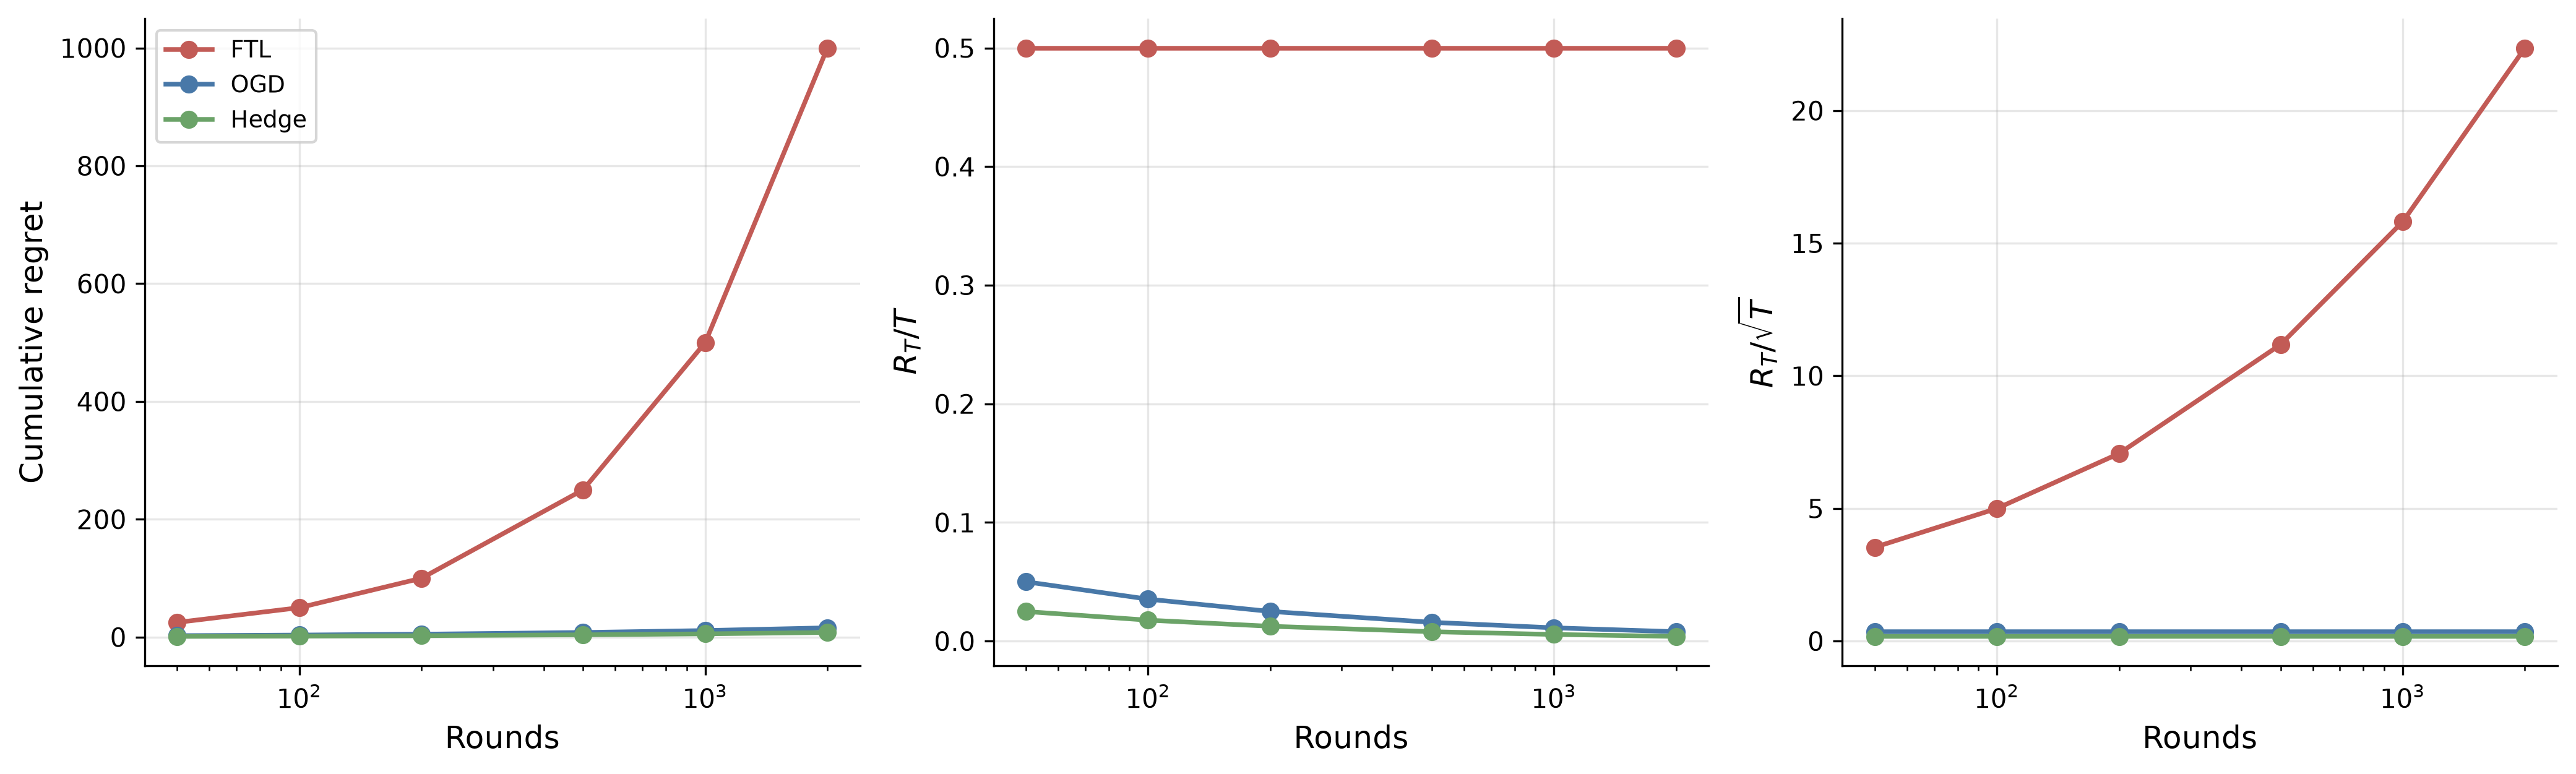
\includegraphics[width=0.98\textwidth]{../ch07a_online_optimization/sims/stability_regret.png}
\caption{Advance power procurement under alternating contract losses. The allocation problem is also a one-state, one-period MDP whose policy assigns probability to the two contracts. FTL follows the past leader and incurs linear regret under the stated tie-breaking rule. Projected gradient descent and Hedge regularize consecutive allocations. The complete loss sequence is fixed before any method runs.}
\label{fig:online_stability}
\end{figure}

\subsection{The one-period connection to reinforcement learning}
\label{sec:online_one_period_mdp}

A one-state, one-period MDP has no continuation value. Let $\mathcal S=\{s\}$, let $\mathcal A$ be a finite action set, and terminate the episode immediately after the action. A stochastic policy is a probability vector
\[
\pi_t(\cdot\mid s)\in\Delta(\mathcal A).
\]
If action $a$ has loss $\ell_t(a)$, the policy's expected loss is
\begin{equation}
\mathbb E_{\pi_t}[\ell_t(A_t)]
=
\sum_{a\in\mathcal A}\pi_t(a\mid s)\ell_t(a)
=
\langle \pi_t,\ell_t\rangle.
\label{eq:one_step_policy_loss}
\end{equation}
This is online linear optimization on the probability simplex. The online decision $x_t$ is the policy vector $\pi_t$, and the MDP's state-action occupancy is the same vector because there is only one state and one period.

The equivalence includes the performance benchmark. The best fixed policy in hindsight solves
\begin{equation}
\min_{\pi\in\Delta(\mathcal A)}
\sum_{t=1}^T\langle\pi,\ell_t\rangle.
\label{eq:one_step_policy_comparator}
\end{equation}
Because the objective is linear, a deterministic action attains the minimum. Regret against the best fixed policy is therefore exactly regret against the best fixed action. No Bellman recursion is required because there is no future state.

The power-procurement simulation implements projected gradient descent twice: first as an online allocation and then as a policy update in the one-state MDP. At every round the action probabilities coincide, and equation~\eqref{eq:one_step_policy_loss} gives the same expected loss. The maximum decision and value discrepancies over 2,000 rounds are both zero to machine precision. The two labels describe the same mathematical problem, not two algorithms with similar behavior.

\subsubsection{Geometry on a probability simplex}
\label{sec:online_entropy_geometry}

Euclidean projection is not the only way to stabilize an update. Let $\psi$ be a differentiable strictly convex function and define its Bregman divergence
\begin{equation}
D_\psi(x,y)
=
\psi(x)-\psi(y)-\langle\nabla\psi(y),x-y\rangle.
\label{eq:online_bregman}
\end{equation}
Online mirror descent updates
\begin{equation}
x_{t+1}
=
\argmin_{x\in\mathcal X}
\left\{
\eta\langle g_t,x\rangle+D_\psi(x,x_t)
\right\}.
\label{eq:online_mirror_descent}
\end{equation}
The first term responds to the new loss. The second measures how far the next decision moves in geometry chosen for the feasible set.

On a probability simplex, the negative-entropy function
\[
\psi(x)=\sum_i x_i\log x_i
\]
produces relative entropy. With a linear loss and no constraints beyond the simplex, equation~\eqref{eq:online_mirror_descent} becomes
\begin{equation}
x_{t+1}(a)
=
\frac{x_t(a)\exp[-\eta\ell_t(a)]}
{\sum_bx_t(b)\exp[-\eta\ell_t(b)]}.
\label{eq:hedge_update}
\end{equation}
This is the Hedge update. A high-loss action loses probability multiplicatively rather than by a fixed Euclidean amount. The same geometry will later be applied to state-action flows, which are also nonnegative probability masses.

\subsection{Chosen-action feedback: the bandit boundary}
\label{sec:online_bandit_boundary}

The equivalence above assumes that the full vector $\ell_t$ is observed after each round. A farmers' market choosing among $A$ stall layouts may instead observe congestion and merchant sales only under the layout actually used. The feasible set is still $\Delta(\mathcal A)$, and the expected loss is still equation~\eqref{eq:one_step_policy_loss}. What changes is the information available for the update.

Under full information, the learner observes $\ell_t(a)$ for every layout. Under chosen-action, or bandit, feedback, it draws $A_t\sim\pi_t$ and observes only $\ell_t(A_t)$. The missing vector can be estimated by
\begin{equation}
\widehat\ell_t(a)
=
\frac{\ell_t(A_t)\indicator{A_t=a}}
{\pi_t(a\mid s)}.
\label{eq:online_importance_loss}
\end{equation}
Conditional on the probabilities selected before the draw,
\begin{equation}
\mathbb E_t[\widehat\ell_t(a)]
=
\sum_b\pi_t(b\mid s)
\frac{\ell_t(b)\indicator{b=a}}{\pi_t(a\mid s)}
=
\ell_t(a).
\label{eq:online_importance_unbiased}
\end{equation}
The estimate is unbiased, but its magnitude contains $1/\pi_t(a\mid s)$. An action assigned very little probability is observed rarely and receives a large update when it is observed. Explicit exploration keeps every denominator away from zero.

Exp3 inserts the importance-weighted vector into an exponential-weight update and mixes the resulting probabilities with a uniform distribution \citep{auer2002nonstochastic}. Its classical expected regret is of order
\begin{equation}
O\!\left(\sqrt{TA\log A}\right),
\label{eq:exp3_regret_order}
\end{equation}
whereas full-information Hedge has order $O(\sqrt{T\log A})$. The extra dependence on $A$ is the cost of estimating losses at layouts that were not selected.

Figure~\ref{fig:online_feedback} uses one pre-generated sequence of layout losses for both feedback protocols. Hedge receives the full vector. Exp3 receives only the selected coordinate and is randomized independently in 200 replications. Increasing the number of layouts from five to ten raises the mean squared loss-estimation error from $2.52$ to $4.25$. At $T=1{,}500$, mean regret is $75.50$ for five-layout Exp3 and $87.61$ for ten-layout Exp3, compared with $32.92$ and $34.66$ for full-information Hedge.

\begin{figure}[htbp]
\centering
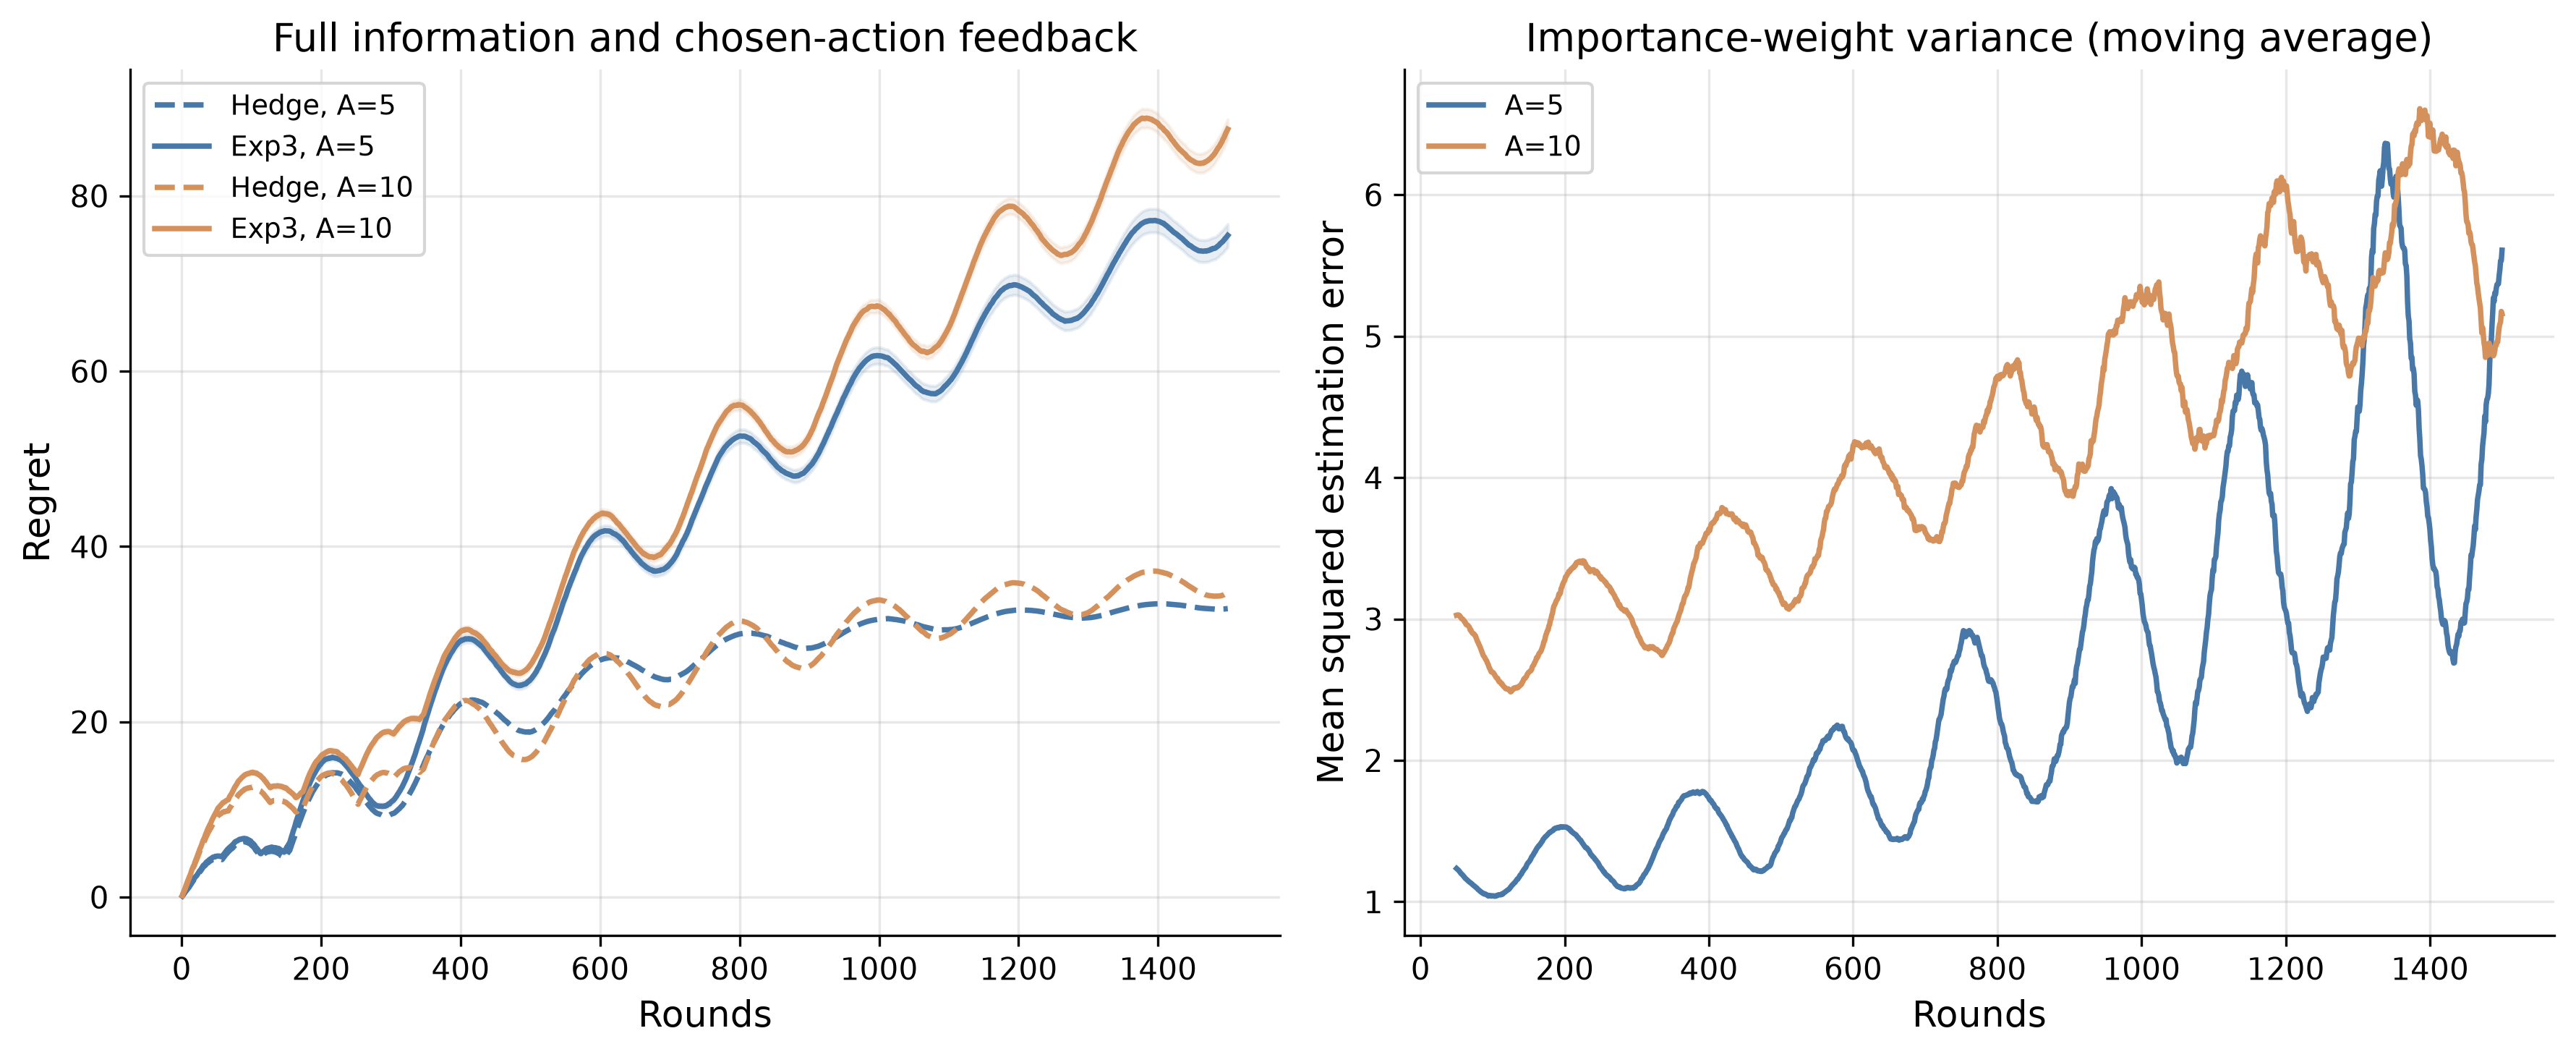
\includegraphics[width=0.96\textwidth]{../ch07a_online_optimization/sims/feedback_regret.png}
\caption{Market-stall layout as a one-period MDP. Dashed curves use Hedge after observing every layout loss. Solid curves use Exp3 after observing only the selected layout. Shading gives 95 percent Monte Carlo intervals across 200 independent algorithm randomizations; the exogenous loss sequence is common to all methods.}
\label{fig:online_feedback}
\end{figure}

An adversarial bandit is therefore online linear optimization with partial feedback and also a one-state, one-period MDP. A contextual bandit adds an observed covariate before the action, but in its standard formulation the action does not change the distribution of later contexts. The substantive break from bandits occurs when an action changes the state in which later rewards and information arrive. Section~\ref{section:bandits} develops stochastic demand learning and dynamic pricing; the present chapter uses the bandit boundary only to locate the first step from online optimization toward RL.

\subsection{Controlled states change the comparator}
\label{sec:online_controlled_states}

Suppose a farm chooses whether to harvest intensively or rest a field. Harvesting affects current output and next season's soil condition. A policy used from the first season therefore generates a different sequence of states from a policy introduced after the field has already been depleted. Evaluating every comparator on the learner's realized soil states ignores this difference.

Write the controlled state law as
\begin{equation}
S_{t+1}=\Phi(S_t,\pi_t,\xi_t),
\label{eq:online_controlled_state_law}
\end{equation}
where $\xi_t$ contains shocks outside the learner's control. If the sequence $\pi_1,\ldots,\pi_{t-1}$ has generated the current state, ordinary external regret would compare
\begin{equation}
\sum_{t=1}^T
\ell\!\left(\pi_t,S_t[\pi_1,\ldots,\pi_{t-1}]\right)
-
\inf_{\pi\in\Pi}
\sum_{t=1}^T
\ell\!\left(\pi,S_t[\pi_1,\ldots,\pi_{t-1}]\right).
\label{eq:online_realized_state_regret}
\end{equation}
The comparator in the second term is inserted into states created by the learner. It is not evaluated under the states it would have created if used throughout.

\emph{Policy regret} changes the second state path:
\begin{equation}
R_T^{\mathrm{pol}}
=
\sum_{t=1}^T
\ell\!\left(\pi_t,S_t[\pi_1,\ldots,\pi_{t-1}]\right)
-
\inf_{\pi\in\Pi}
\sum_{t=1}^T
\ell\!\left(\pi,S_t[\pi,\ldots,\pi]\right).
\label{eq:online_policy_regret}
\end{equation}
The first term remains the learner's realized loss. The comparator is now deployed counterfactually from the initial state. This is the same comparison used by RL regret against a fixed policy: each policy is evaluated under its own induced state distribution.

\subsubsection{A two-state soil model}

The soil simulation has states fertile and depleted and actions harvest and rest. Rewards are
\begin{center}
\begin{tabular}{lrr}
\toprule
 & Harvest & Rest \\
\midrule
Fertile & $1.0$ & $0.2$ \\
Depleted & $0.0$ & $0.2$ \\
\bottomrule
\end{tabular}
\end{center}
Harvesting makes the next state depleted; resting makes it fertile. The model is deterministic:
\begin{equation}
\Pr(S_{t+1}=\text{depleted}\mid S_t,\text{harvest})=1,
\qquad
\Pr(S_{t+1}=\text{fertile}\mid S_t,\text{rest})=1.
\label{eq:soil_transitions}
\end{equation}
The policy class contains the four deterministic Markov rules mapping the two states into the two actions. Starting from fertile soil, the rule ``harvest when fertile, rest when depleted'' rotates between the two states and is the best fixed Markov policy in the class.

The learner used for the diagnostic always harvests. It receives reward one in the first season and zero thereafter. On this realized path, the field is depleted from season two onward. Evaluating the rotation rule on those same states assigns it reward $0.2$ in every later season and produces external regret $23.8$ after 120 seasons. Deploying the rotation rule from the beginning instead makes the state alternate; it earns $1.0,0.2,1.0,0.2,\ldots$ and produces policy regret $71.0$ against the always-harvest learner.

\begin{figure}[htbp]
\centering
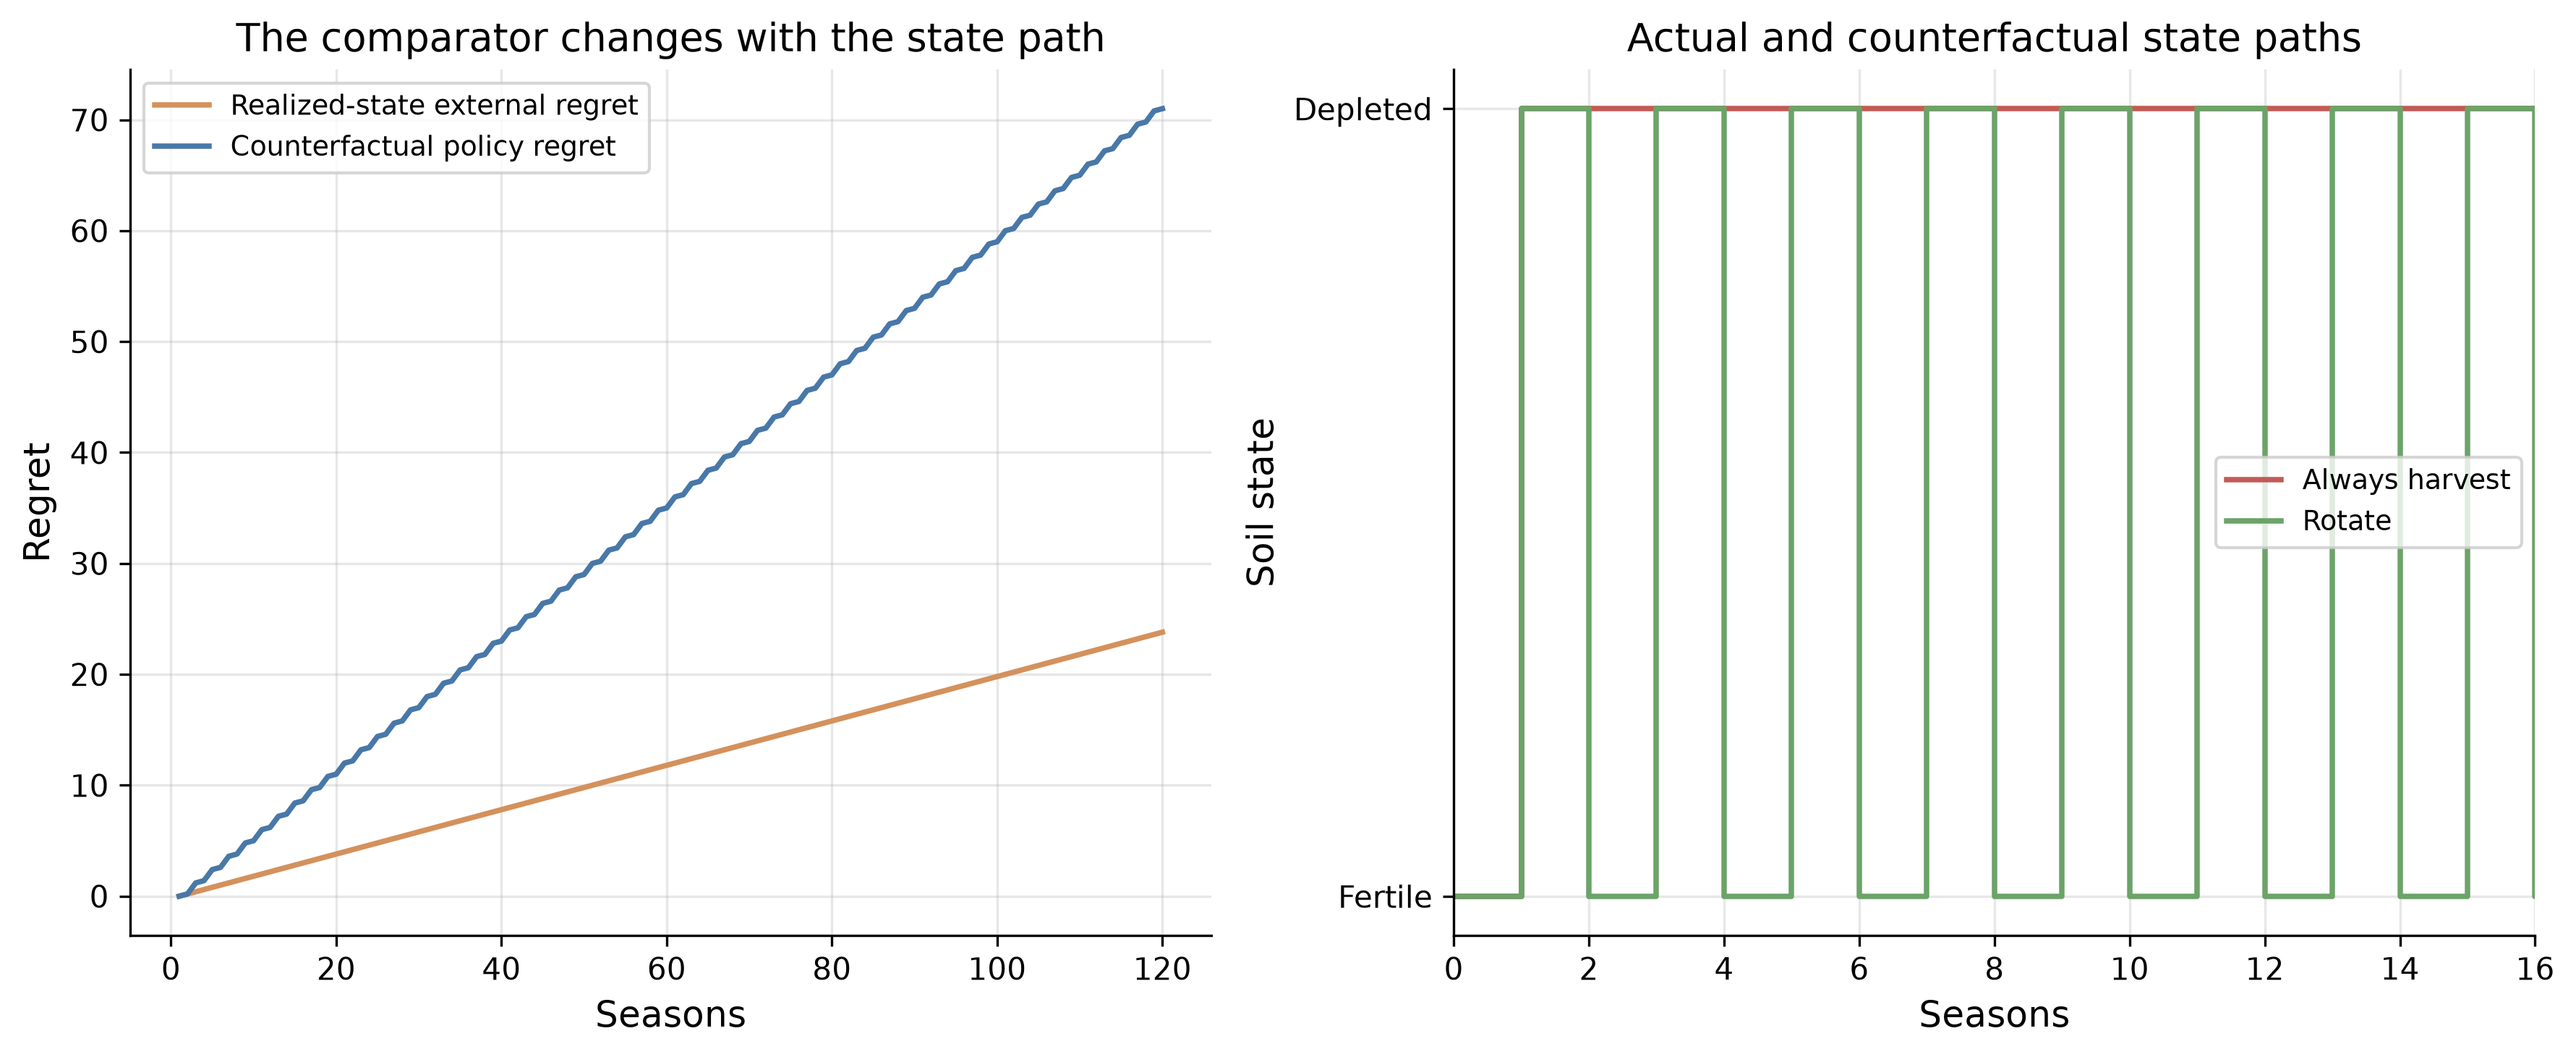
\includegraphics[width=0.96\textwidth]{../ch07a_online_optimization/sims/soil_policy_regret.png}
\caption{Realized-state and counterfactual comparison in the soil MDP. The left panel evaluates the same always-harvest learner under two comparators. The right panel displays the first sixteen seasons of the actual depleted path and the state path generated by the rotation policy from the initial state.}
\label{fig:online_soil_policy_regret}
\end{figure}

The gap is not estimation error. Rewards and transitions are known exactly, and the best Markov comparator is found by enumerating the four policies. The difference comes entirely from the state distribution assigned to the comparator. Ordinary external regret is appropriate in the one-period problem because actions create no later state. Once states are controlled, equation~\eqref{eq:online_policy_regret} is the relevant object.

\subsubsection{Dynamic stability}

\citet{bhatiaSridharan2020} study this issue for a general class of online problems with dynamics. Their analysis separates two obstacles. The first is ordinary online complexity: how difficult it is to compete with the policy class when counterfactual losses are revealed sequentially. The second is \emph{dynamic stability}: how much the current policy's loss changes because earlier policies, rather than the current policy, generated the state in which it is deployed.

In their notation, a regularized empirical-risk minimizer has a minimax-value bound of the form
\begin{equation}
V_T
\leq
\sum_{t=1}^T\beta_{\mathrm{RERM},t}
+
2\mathfrak R_T^{\mathrm{seq}}(\ell^\Phi\circ\Pi)
+
2\lambda\sup_{\pi\in\Pi}\Omega(\pi).
\label{eq:online_dynamics_bound}
\end{equation}
The terms require translation. The sequence $\beta_{\mathrm{RERM},t}$ bounds the loss change caused by deploying the current policy after a history generated by other policies. The sequential Rademacher complexity $\mathfrak R_T^{\mathrm{seq}}$ measures the richness of the counterfactual loss class under adaptive data; it is the dynamic analogue of a statistical complexity penalty. The final term is the contribution of the regularizer $\Omega$. When loss does not depend on state, the dynamic-stability term vanishes and the problem returns to ordinary online learning.

Equation~\eqref{eq:online_dynamics_bound} is a learnability characterization, not a tabular RL algorithm. Its role here is to locate the obstruction. The next section uses the known transition law to encode the state path directly in the decision variable. That representation turns the counterfactual comparison into ordinary regret over a constrained set of state-action flows.

\subsection{Known transitions: online optimization over occupancies}
\label{sec:online_known_transitions}

Consider an episodic MDP with finite state space $\mathcal S$, finite action space $\mathcal A$, horizon $H$, initial distribution $\rho$, and known stage-dependent transition kernels
\[
P_h(s'\mid s,a),
\qquad h=1,\ldots,H-1.
\]
Before episode $k$, the learner selects a Markov policy $\pi_k=(\pi_{k,1},\ldots,\pi_{k,H})$. The environment then supplies stage losses $\ell_{k,h}(s,a)$. The episode loss is
\begin{equation}
J_k(\pi_k)
=
\mathbb E_{\pi_k,P}
\left[
\sum_{h=1}^H\ell_{k,h}(S_h,A_h)
\right].
\label{eq:online_mdp_episode_loss}
\end{equation}
Transitions are fixed across episodes, while the loss functions may change. This is the online MDP studied by \citet{ziminNeu2013}. It differs from the usual introductory RL problem, where one reward function is fixed and the transition law is initially unknown.

\subsubsection{State-action occupancies}

Use the episodic occupancy notation already used in Section~\ref{section:offline_rl}:
\begin{equation}
d_{k,h}^{\pi}(s,a)
=
\Pr_{\pi,P}(S_h=s,A_h=a).
\label{eq:online_episodic_occupancy}
\end{equation}
The array $d^\pi=(d_1^\pi,\ldots,d_H^\pi)$ records both the policy's action probabilities and the state distribution those actions induce. Its entries are nonnegative and obey
\begin{align}
\sum_a d_1^\pi(s,a)
&=
\rho(s),
\label{eq:online_flow_initial}\\
\sum_a d_{h+1}^\pi(s,a)
&=
\sum_{s',a'}
d_h^\pi(s',a')P_h(s\mid s',a'),
\qquad h=1,\ldots,H-1.
\label{eq:online_flow_transition}
\end{align}
The first equation assigns the initial mass. The second says that mass entering state $s$ at stage $h+1$ must equal the mass sent there from every state-action pair at stage $h$. These are the finite-horizon counterparts of the discounted flow equations in Section~\ref{sec:planning_learning}.

Let $\mathcal D(P)$ denote the set of nonnegative arrays satisfying equations~\eqref{eq:online_flow_initial}--\eqref{eq:online_flow_transition}. The transition law appears in the definition of this set; known $P$ is therefore not a cosmetic assumption. Because the restrictions are linear, $\mathcal D(P)$ is a convex polytope.

Every Markov policy produces an element of $\mathcal D(P)$. The converse also holds. Given a feasible $d$, define
\begin{equation}
\pi_h^d(a\mid s)
=
\frac{d_h(s,a)}
{\sum_b d_h(s,b)}
\label{eq:online_occupancy_policy}
\end{equation}
whenever the denominator is positive. At a state with zero occupancy, choose any action distribution; the choice cannot affect the flow because the state is never reached. Substituting equation~\eqref{eq:online_occupancy_policy} into the forward state recursion recovers $d$.

\subsubsection{A two-period flow calculation}

Before considering online updates, it is useful to compute one occupancy by hand. Take the first two periods of the timed-entry model. The museum begins quiet with probability one. In period one it admits with probability $p$ and holds with probability $1-p$. Using the two quiet-state rows of equation~\eqref{eq:online_museum_transitions}, the period-two state probabilities are
\begin{align}
\Pr(S_2=\text{quiet})
&=(1-p)(0.90)+p(0.35)=0.90-0.55p,\\
\Pr(S_2=\text{busy})
&=(1-p)(0.10)+p(0.55)=0.10+0.45p,\\
\Pr(S_2=\text{crowded})
&=p(0.10)=0.10p.
\label{eq:online_two_period_state_mass}
\end{align}
Suppose the period-two policy admits with probabilities $u_q,u_b,u_c$ in the three states. The nonzero occupancies are then
\begin{align*}
d_1(\text{quiet},\text{hold})&=1-p,
&d_1(\text{quiet},\text{admit})&=p,\\
d_2(\text{quiet},\text{admit})&=(0.90-0.55p)u_q,
&d_2(\text{quiet},\text{hold})&=(0.90-0.55p)(1-u_q),\\
d_2(\text{busy},\text{admit})&=(0.10+0.45p)u_b,
&d_2(\text{busy},\text{hold})&=(0.10+0.45p)(1-u_b),\\
d_2(\text{crowded},\text{admit})&=0.10pu_c,
&d_2(\text{crowded},\text{hold})&=0.10p(1-u_c).
\end{align*}
Summing actions in the second period recovers equation~\eqref{eq:online_two_period_state_mass}. The three state masses sum to one for every $p\in[0,1]$.

This calculation shows what the occupancy decision contains. Changing $p$ changes both the first-period action mass and every second-period state mass. The expected two-period loss is nevertheless the linear expression
\begin{equation}
\sum_a d_1(\text{quiet},a)\ell_1(\text{quiet},a)
+
\sum_{s,a}d_2(s,a)\ell_2(s,a).
\label{eq:online_two_period_linear_loss}
\end{equation}
The nonlinearity has moved from the objective into the feasible relationship among the entries of $d$. This is why optimizing separately over $p,u_q,u_b,u_c$ is not generally a convex problem in primitive policy probabilities, while optimizing over the complete feasible array $d$ is linear.

Conversely, suppose a solver returns the entries above without reporting $p$ or the $u$'s. Equation~\eqref{eq:online_occupancy_policy} recovers
\[
p=d_1(\text{quiet},\text{admit}),
\qquad
u_s=\frac{d_2(s,\text{admit})}{\sum_a d_2(s,a)}.
\]
The ratios are undefined only at period-two states having zero mass, where the action cannot influence expected loss. Thus the flow representation retains all behaviorally relevant policy information.

\subsubsection{The exact reduction}

Linearity of expectation converts equation~\eqref{eq:online_mdp_episode_loss} into
\begin{align}
J_k(\pi)
&=
\sum_{h=1}^H\sum_{s,a}
\Pr_{\pi,P}(S_h=s,A_h=a)\ell_{k,h}(s,a)
\nonumber\\
&=
\sum_{h,s,a}
d_h^\pi(s,a)\ell_{k,h}(s,a)
\nonumber\\
&=
\langle d^\pi,\ell_k\rangle.
\label{eq:online_occupancy_identity}
\end{align}
The policy changes the state distribution, but that response is already contained in $d^\pi$. Expected loss is linear in the enlarged decision variable.

Regret against the best fixed Markov policy in hindsight is consequently
\begin{align}
R_K
&=
\sum_{k=1}^KJ_k(\pi_k)
-
\min_\pi\sum_{k=1}^KJ_k(\pi)
\nonumber\\
&=
\sum_{k=1}^K\langle d_k,\ell_k\rangle
-
\min_{d\in\mathcal D(P)}
\sum_{k=1}^K\langle d,\ell_k\rangle.
\label{eq:online_mdp_occupancy_regret}
\end{align}
Equation~\eqref{eq:online_mdp_occupancy_regret} is an equality of optimization problems. It is online linear optimization with feasible set $\mathcal D(P)$. Unlike the realized-state comparator in equation~\eqref{eq:online_realized_state_regret}, each feasible comparator carries the state distribution generated by its own actions.

The $H=1$, one-state case recovers Section~\ref{sec:online_one_period_mdp}. The only flow constraint is $\sum_a d_1(s,a)=1$, so $\mathcal D(P)=\Delta(\mathcal A)$ and $d_1(s,a)=\pi(a\mid s)$. Occupancy optimization is therefore the multi-period extension of the action-probability update, with flow conservation accounting for controlled future states.

\subsubsection{Relative-entropy policy search}
\label{sec:online_oreps}

Applying the mirror update in equation~\eqref{eq:online_mirror_descent} to $\mathcal D(P)$ with negative-entropy geometry gives
\begin{equation}
d_{k+1}
=
\argmin_{d\in\mathcal D(P)}
\left\{
\eta\langle d,\widehat\ell_k\rangle
+
D_{\mathrm{KL}}(d\Vert d_k)
\right\},
\label{eq:online_oreps_update}
\end{equation}
where
\begin{equation}
D_{\mathrm{KL}}(d\Vert d_k)
=
\sum_{h,s,a}
\left[
d_h(s,a)\log\frac{d_h(s,a)}{d_{k,h}(s,a)}
-d_h(s,a)+d_{k,h}(s,a)
\right].
\label{eq:online_flow_kl}
\end{equation}
The linear term favors flows with low observed loss. The relative-entropy term limits how much probability mass moves between consecutive episode occupancies. The flow constraints ensure that the result remains implementable by a policy. The next policy is recovered with equation~\eqref{eq:online_occupancy_policy}.

\citet{ziminNeu2013} call the algorithm O-REPS, for Online Relative Entropy Policy Search. Their MDP is layered and loop-free: each state belongs to one stage, transitions move only to the next layer, and an episode has $H$ layers. Let $S_{\mathrm{tot}}$ be the number of state copies across all layers and let $A=|\mathcal A|$. With losses in $[0,1]$ and known transitions, their full-information expected-regret bound translates to
\begin{equation}
R_K
\leq
2H
\sqrt{
K\log\!\left(\frac{S_{\mathrm{tot}}A}{H}\right)
}.
\label{eq:online_oreps_full_bound}
\end{equation}
Under their trajectory-feedback model, where losses are observed only at visited state-action pairs, importance weighting gives
\begin{equation}
R_K
\leq
2
\sqrt{
HS_{\mathrm{tot}}AK
\log\!\left(\frac{S_{\mathrm{tot}}A}{H}\right)
}.
\label{eq:online_oreps_bandit_bound}
\end{equation}
The second bound contains the same estimation cost encountered in the one-period bandit, now multiplied by the number of state-action locations at which loss may need to be inferred. The bounds do not cover unknown transitions; $P$ is used both to define $\mathcal D(P)$ and to compute the update.

\subsubsection{Timed-entry admissions}
\label{sec:online_museum}

A museum divides each day into twelve admission periods. The operating state is quiet, busy, or crowded. At each period it either holds admissions or admits the next group. The unnormalized loss in day $k$ is
\begin{equation}
\ell_k(s,a)
=
d_s+\kappa a-a v_km_s,
\label{eq:online_museum_loss}
\end{equation}
with
\[
d=(0,0.15,0.90),
\qquad
m=(1,0.60,0.15),
\qquad
\kappa=0.25.
\]
The term $d_s$ is the visitor-experience and operating cost of crowding. Admitting a group has service cost $\kappa$ and day-specific value $v_km_s$, which is highest in the quiet state. The value $v_k$ alternates in blocks of fifty days between $1.25$ and $0.55$. A single affine transformation places all simulated losses in $[0,1]$ without changing their ordering.

Holding and admitting have known transition matrices
\begin{equation}
P_0=
\begin{pmatrix}
.90&.10&0\\
.35&.55&.10\\
0&.45&.55
\end{pmatrix},
\qquad
P_1=
\begin{pmatrix}
.35&.55&.10\\
.05&.45&.50\\
0&.10&.90
\end{pmatrix}.
\label{eq:online_museum_transitions}
\end{equation}
Rows index the current state and columns the next state. Admitting raises the probability of moving toward crowding and makes the crowded state more persistent. The immediate value of admission must therefore be compared with the continuation cost created by the induced state distribution.

Four rules are evaluated over 300 days.
\begin{enumerate}
\item The myopic rule minimizes the current-period loss at each state and ignores the next-state distribution.
\item The state-blind learner uses one admission probability in every state and updates it by exponential weights.
\item Per-state Hedge keeps separate action weights at quiet, busy, and crowded states but updates them from immediate losses, without continuation values.
\item O-REPS updates the complete occupancy array with equation~\eqref{eq:online_oreps_update}.
\end{enumerate}
The hindsight comparator is the exact fixed Markov policy minimizing the sum of all 300 daily losses. Because transitions are common across days, it is obtained by backward induction on the average loss. All methods and the comparator use the same twelve-period MDP.

The O-REPS update is solved directly as a convex program with the linear flow equations and the relative-entropy objective. No generic RL library is involved. Two numerical checks compare the optimization and MDP representations. The maximum flow-conservation residual is $2.78\times10^{-16}$. Evaluating every policy once by the occupancy inner product and once by ordinary Bellman recursion gives a maximum discrepancy of $7.11\times10^{-15}$.

\begin{figure}[htbp]
\centering
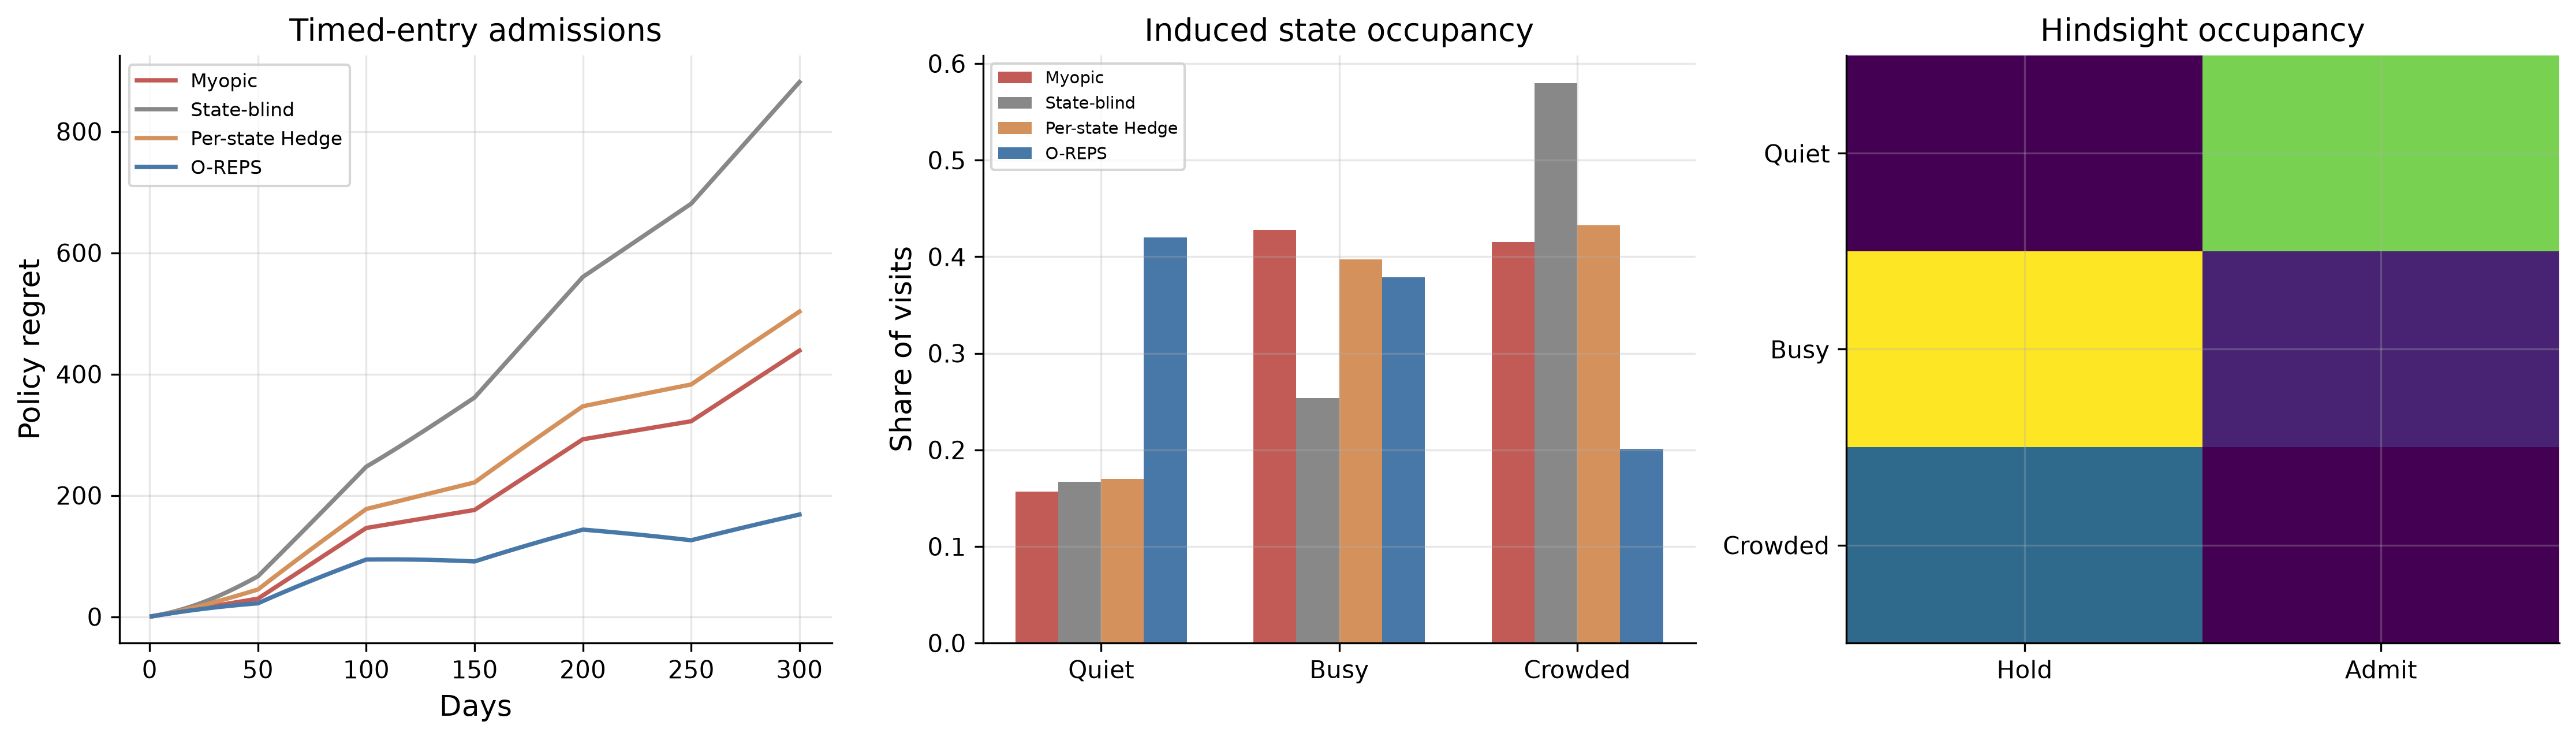
\includegraphics[width=0.99\textwidth]{../ch07a_online_optimization/sims/occupancy_online_mdp.png}
\caption{The timed-entry MDP and its occupancy formulation. The left panel reports regret against the exact best fixed Markov policy in hindsight. The middle panel reports the state distribution induced by each method. The right panel gives the comparator's state-action occupancy summed over the twelve periods.}
\label{fig:online_occupancy}
\end{figure}

\begin{table}[htbp]
\centering
\caption{Timed-entry admissions with known transitions. Admission rates condition on visits to the named state.}
\label{tab:online_optimization_summary}
\small
\begin{tabular}{lrrrrr}
\toprule
Method & Final regret & Crowded share & Quiet admit & Busy admit & Crowded admit \\
\midrule
Myopic & 438.73 & 0.415 & 1.000 & 1.000 & 0.000 \\
State-blind & 881.42 & 0.580 & 0.905 & 0.920 & 0.945 \\
Per-state Hedge & 502.99 & 0.432 & 0.957 & 0.940 & 0.227 \\
O-REPS & 168.46 & 0.201 & 0.549 & 0.293 & 0.279 \\
\bottomrule
\end{tabular}
% maximum occupancy flow residual: 2.776e-16
% maximum Bellman/occupancy value residual: 7.105e-15

\end{table}

The myopic rule admits whenever immediate value exceeds immediate cost and spends $41.5$ percent of periods crowded. Its final regret is $438.73$. Per-state Hedge also omits continuation values and ends at $502.99$. The state-blind rule cannot condition on congestion, admits with nearly the same probability in every state, and ends at $881.42$. O-REPS internalizes the flow response: it admits at rates $0.549$, $0.293$, and $0.279$ in the quiet, busy, and crowded states, spends $20.1$ percent of periods crowded, and ends at regret $168.46$.

These finite-sample differences are not estimates of the asymptotic rates in equations~\eqref{eq:online_oreps_full_bound}--\eqref{eq:online_oreps_bandit_bound}. Their purpose is to verify the reduction on identical primitives. The MDP calculation and the online linear objective agree policy by policy; the algorithms differ in whether their decision variable respects the complete state-flow response.

\subsection{A fixed MDP solved by no-regret updates}
\label{sec:online_fixed_mdp}

The preceding section studies repeated deployment when the episode loss can change. A second use of online learning begins with one stationary discounted MDP. Rewards and transitions are fixed. The online sequence is created inside the numerical method, and regret controls the quality of the policy returned by that method. This is an optimization algorithm for an MDP, not an adversarial online MDP.

Use the normalized discounted occupancy from Appendix~\ref{appendix:mathprelim}:
\begin{equation}
d_\rho^\pi(s,a)
=
(1-\gamma)
\mathbb E_{\rho,\pi}
\left[
\sum_{t=0}^\infty
\gamma^t\indicator{S_t=s,A_t=a}
\right].
\label{eq:online_discounted_occupancy}
\end{equation}
Its entries sum to one. The expected reward under this distribution is the normalized discounted value,
\begin{equation}
\sum_{s,a}d_\rho^\pi(s,a)r(s,a)
=
(1-\gamma)V^\pi(\rho).
\label{eq:online_normalized_value}
\end{equation}

The factor $1-\gamma$ differs from the episodic convention in equation~\eqref{eq:online_episodic_occupancy}. In an $H$-period episode, each stage occupancy sums to one and the full array sums to $H$. In the discounted problem, multiplication by $1-\gamma$ makes the complete infinite-horizon array sum to
\[
(1-\gamma)\sum_{t=0}^\infty\gamma^t=1.
\]
The normalized array can therefore be treated as a probability distribution over a randomly selected discounted state-action visit. An unnormalized discounted occupancy would omit $1-\gamma$, sum to $1/(1-\gamma)$, and have objective $V^\pi(\rho)$ directly. Both conventions describe the same policies, but their linear-program objectives and regret scales differ by $1-\gamma$.

The finite-horizon and discounted reductions also answer different substantive questions. In the episodic online MDP, a day-specific loss array $\ell_k$ arrives after policy $\pi_k$ is selected, and the comparator is the best fixed policy across days. In the discounted program, $r$ and $P$ are fixed. The iterates $V_n$ and $d_n$ are numerical proposals, not policies deployed into a changing environment. The online objectives are gradients of one stationary saddle function.

\subsubsection{The Bellman linear programs}

The occupancy formulation of the fixed control problem is
\begin{align}
\max_{d\geq0}\quad&
\sum_{s,a}d(s,a)r(s,a)
\label{eq:online_discounted_primal}\\
\text{subject to}\quad&
\sum_a d(s,a)
=
(1-\gamma)\rho(s)
+
\gamma\sum_{s',a'}
P(s\mid s',a')d(s',a')
\quad\text{for every }s.
\nonumber
\end{align}
The constraints are discounted flow conservation. The mass initially injected at state $s$ is $(1-\gamma)\rho(s)$; the remaining mass arrives from discounted transitions out of other state-action pairs.

The dual program searches over value functions:
\begin{align}
\min_V\quad&
(1-\gamma)\sum_s\rho(s)V(s)
\label{eq:online_discounted_dual}\\
\text{subject to}\quad&
V(s)
\geq
r(s,a)+\gamma\sum_{s'}P(s'\mid s,a)V(s')
\quad\text{for every }(s,a).
\nonumber
\end{align}
The constraints are Bellman inequalities. At an optimum, an action with positive occupancy has a binding inequality by complementary slackness. Dividing the common primal and dual optimum by $1-\gamma$ recovers $V^*(\rho)$.

This primal-dual pair was introduced as a characterization of optimal control in Section~\ref{sec:planning_learning}. Its role here is computational. Move the flow equalities into a Lagrangian,
\begin{equation}
L(V,d)
=
(1-\gamma)\rho^\top V
+
\sum_{s,a}d(s,a)
\left[
r(s,a)
+\gamma\sum_{s'}P(s'\mid s,a)V(s')
-V(s)
\right].
\label{eq:online_bellman_lagrangian}
\end{equation}
On suitable compact domains, solving the MDP is equivalent to finding a saddle point
\begin{equation}
\min_V\max_d L(V,d).
\label{eq:online_bellman_saddle}
\end{equation}
The occupancy player places mass on state-action pairs with positive Bellman advantage. The value player changes $V$ to reduce those violations while pricing the flow constraints.

\subsubsection{From online regret to a saddle point}

Suppose the value player generates $V_1,\ldots,V_N$ and the occupancy player generates $d_1,\ldots,d_N$. In round $n$, each player treats $L(V_n,d_n)$ as its online objective: the value player minimizes and the occupancy player maximizes. Let $R_N^V$ and $R_N^d$ be their external regrets on the chosen compact domains. For the averages
\[
\bar V_N=\frac1N\sum_{n=1}^NV_n,
\qquad
\bar d_N=\frac1N\sum_{n=1}^Nd_n,
\]
bilinearity gives
\begin{equation}
\max_dL(\bar V_N,d)
-
\min_VL(V,\bar d_N)
\leq
\frac{R_N^V+R_N^d}{N}.
\label{eq:online_saddle_regret}
\end{equation}
The left side is the saddle gap. If both regrets grow sublinearly, their average vanishes and the averaged iterates approach a saddle point.

A small saddle gap does not automatically identify which policy should be returned. Normalize the averaged occupancy within each state,
\begin{equation}
\widehat\pi_N(a\mid s)
=
\frac{\bar d_N(s,a)}
{\sum_b\bar d_N(s,b)}.
\label{eq:online_saddle_policy}
\end{equation}
\citet{cheng2020noregret} choose an output-dependent comparator that links the online regret directly to this policy's performance. In their tabular formulation and normalization,
\begin{equation}
V^{\widehat\pi_N}(\rho)
\geq
V^*(\rho)
-
\frac{\operatorname{Regret}_N}{N}.
\label{eq:online_cheng_tabular}
\end{equation}
When the value or occupancy player is restricted to a function class $\Theta$, their analysis adds an approximation term:
\begin{equation}
V^*(\rho)-V^{\widehat\pi_N}(\rho)
\leq
\frac{\operatorname{Regret}_N(\Theta)}{N}
+
\varepsilon_{\Theta,N}.
\label{eq:online_cheng_approximation}
\end{equation}
The first term is controlled by the online algorithm. The second measures whether the chosen function class can represent the comparator needed by the reduction. This separation is useful in large state spaces: changing the optimizer and changing the representation affect different terms.

The theorem does not say that arbitrary iterates of an arbitrary saddle algorithm are good policies. It concerns the specified averaged output, comparator construction, domains, and sampling assumptions. Cheng et al.\ instantiate the reduction with a mirror-descent algorithm and a generative-model oracle. The experiment below uses exact model expectations so that optimization behavior is separated from sampling noise.

\subsubsection{The Engine Replacement MDP}
\label{sec:online_engine_saddle}

The common primitives are those of Section~\ref{engine:model}. A low-mileage engine yields reward $1$ when kept and moves to high mileage with probability $0.5$. A high-mileage engine yields reward $0.2$ when kept and remains worn. Replacement costs $0.5$ and returns either state to low mileage. The discount factor is $\gamma=0.9$. The exact optimal values are
\[
V^*(\text{low})=\frac{155}{29},
\qquad
V^*(\text{high})=\frac{125}{29},
\]
and the optimal policy keeps at low mileage and replaces at high mileage.

Two solvers receive exactly these rewards and transitions. Value iteration applies the Bellman optimality operator from Section~\ref{sec:planning_learning}. The saddle solver applies projected gradient descent to the value player and exponentiated-gradient ascent to the normalized occupancy player in equation~\eqref{eq:online_bellman_lagrangian}. Its reported value and occupancy are averages of all preceding iterates.

\begin{figure}[htbp]
\centering
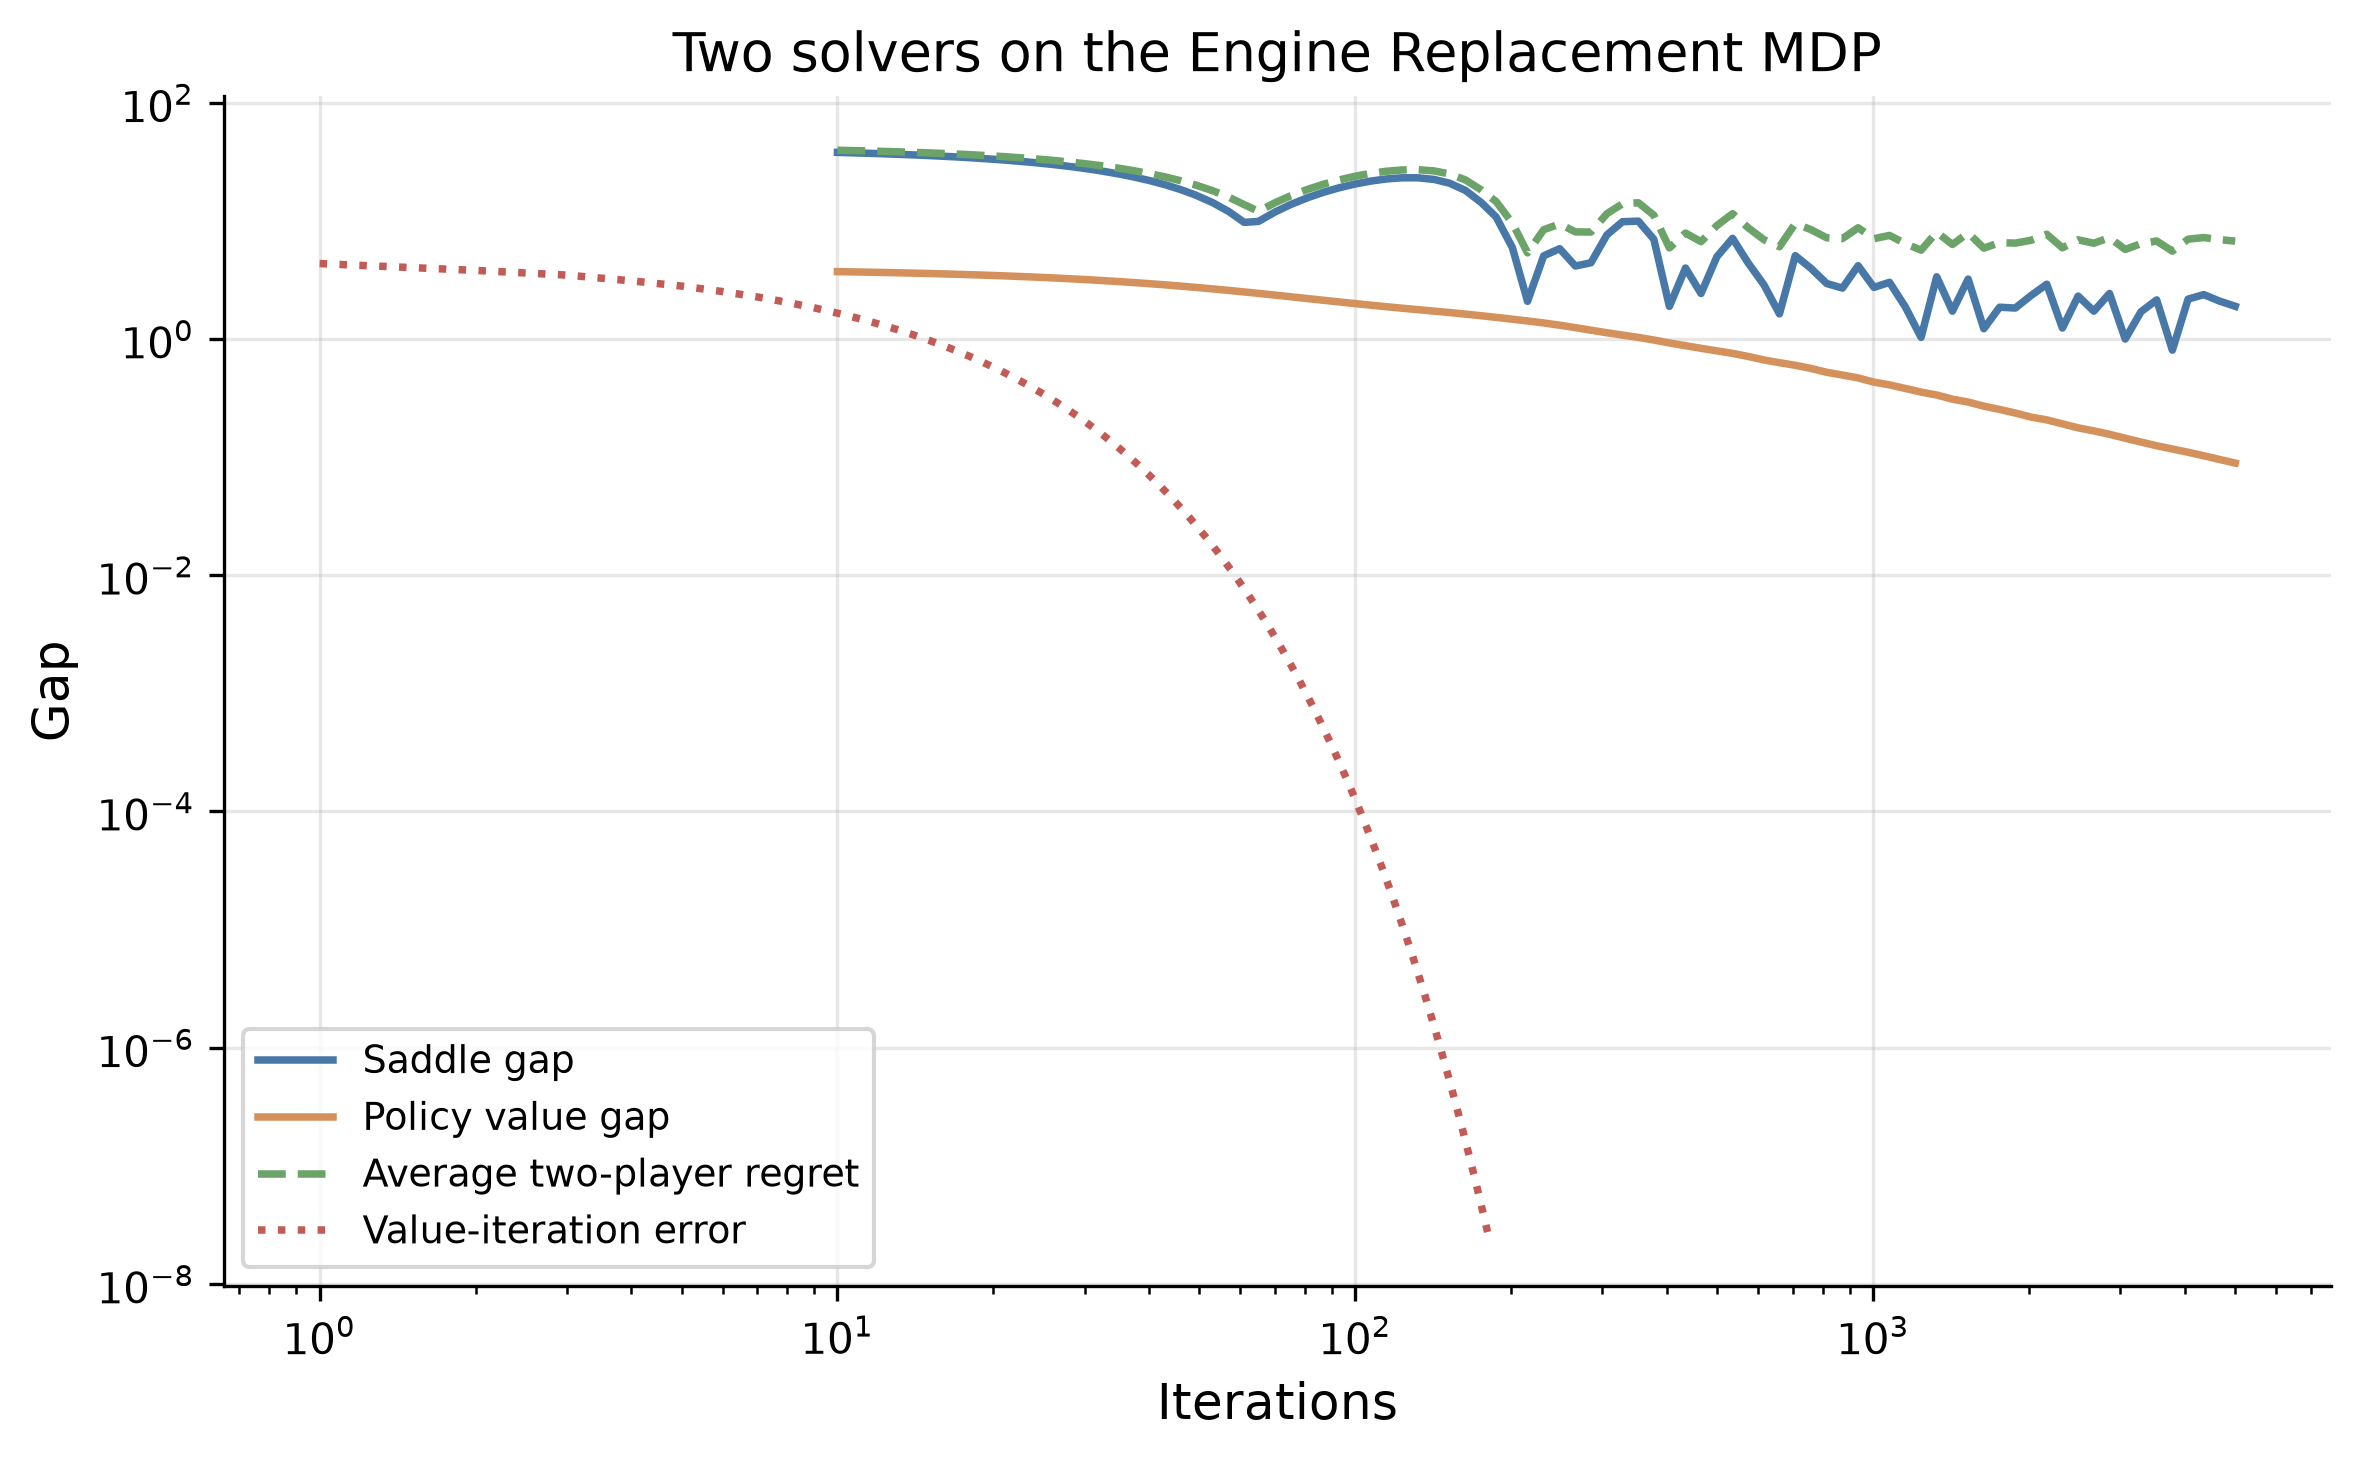
\includegraphics[width=0.80\textwidth]{../ch07a_online_optimization/sims/bellman_no_regret.png}
\caption{Two solution methods on the same Engine Replacement MDP. Value iteration reports distance from the exact value. The no-regret solver reports the policy-value gap, the Bellman saddle gap, and its generic two-player regret certificate. All quantities use exact model expectations.}
\label{fig:online_bellman_solver}
\end{figure}

Value iteration exploits the Bellman contraction and reaches value error $2.75\times10^{-8}$ after 180 iterations. The more general saddle method has policy-value gap $0.089$ after 5,000 iterations; its saddle and generic regret diagnostics are looser. This is not a claim that no-regret dynamics are faster than dynamic programming on a two-state tabular model. The comparison establishes that the same fixed MDP can be solved through either Bellman iteration or an internally generated online-learning problem. The value of the reduction is its modularity: alternative online algorithms and function classes can be inserted while retaining a policy guarantee of the form in equation~\eqref{eq:online_cheng_approximation}.

The distinction between the chapter's two exact connections is now explicit. In equation~\eqref{eq:online_mdp_occupancy_regret}, losses change across deployed episodes and regret is the performance criterion. In equation~\eqref{eq:online_saddle_regret}, the environment is fixed and online regret is an internal convergence certificate for a numerical solver.

\subsection{Unknown transitions: optimization no longer suffices}
\label{sec:online_unknown_transitions}

The occupancy reduction assumes that $\mathcal D(P)$ is known before the decision is made. If $P$ is unknown, the learner does not know which state-action flows are feasible. It also observes transitions only at state-action pairs reached by its policy. The choice of policy therefore determines both current performance and the observations used to estimate the next feasible set.

Three changes occur together.
\begin{enumerate}
\item The flow constraints contain unknown transition probabilities.
\item Losses and transitions may be observed only at visited state-action pairs.
\item Avoiding an uncertain region can prevent the uncertainty from shrinking.
\end{enumerate}
The first is a model-estimation problem. The second is partial feedback. The third is exploration: the sampling distribution is controlled by the policy being learned.

A model-based RL algorithm commonly maintains transition counts $N_k(s,a,s')$ and estimates
\begin{equation}
\widehat P_k(s'\mid s,a)
=
\frac{N_k(s,a,s')}
{\max\{1,N_k(s,a)\}},
\label{eq:online_empirical_transition}
\end{equation}
where $N_k(s,a)=\sum_{s'}N_k(s,a,s')$. A certainty-equivalent learner inserts $\widehat P_k$ into a planner and behaves as if the estimate were correct. This can fail when the current policy does not visit the pairs at which its model is wrong.

Optimistic model-based methods also maintain a set $\mathcal P_k$ of transition laws statistically consistent with the observed counts. They plan using a favorable member of this set, or subtract a bonus from uncertain losses. An uncertain action can then be selected because of what might be learned or earned there, even when its empirical estimate is not currently best. As counts accumulate, confidence sets and bonuses contract.

\subsubsection{Cold-storage maintenance}
\label{sec:online_cold_storage}

A cold-storage operator observes equipment in a normal, strained, or failing state. It can monitor the equipment or perform preventive service. The stage-loss matrix is
\begin{center}
\begin{tabular}{lrr}
\toprule
 & Monitor & Service \\
\midrule
Normal & $0.00$ & $0.24$ \\
Strained & $0.18$ & $0.34$ \\
Failing & $1.00$ & $0.55$ \\
\bottomrule
\end{tabular}
\end{center}
Service is costly in a normal or strained state but reduces the probability of failure. The transition matrices are
\begin{equation}
P_{\mathrm{monitor}}
=
\begin{pmatrix}
.75&.25&0\\
.05&.65&.30\\
0&.05&.95
\end{pmatrix},
\qquad
P_{\mathrm{service}}
=
\begin{pmatrix}
.95&.05&0\\
.60&.38&.02\\
.45&.45&.10
\end{pmatrix}.
\label{eq:online_storage_transitions}
\end{equation}
An episode has twelve maintenance periods and begins in the normal state.

The known-model benchmark receives equation~\eqref{eq:online_storage_transitions} and solves the finite-horizon MDP exactly. This is also the optimizer over the known occupancy set $\mathcal D(P)$. The certainty-equivalent learner estimates each transition row from its own visits and solves the estimated MDP exactly before every episode. For an unvisited state-action pair it initially uses a self-loop, a deliberately simple default that makes the consequences of missing exploration visible.

The optimistic learner uses the same empirical model but subtracts a count-based bonus,
\begin{equation}
b_k(s,a)
=
0.55
\sqrt{
\frac{\log(KSA+1)}
{\max\{1,N_k(s,a)\}}
},
\label{eq:online_storage_bonus}
\end{equation}
from the planning loss. This is an illustrative upper-confidence heuristic rather than an implementation of the minimax algorithms stated below. All three rules are evaluated on trajectories from the same true transition law.

The left panel of Figure~\ref{fig:online_unknown_dynamics} reports regret against the exact expected loss of the known-model policy over 100 replications. The known-model planner has mean final regret $0.02$, statistically indistinguishable from zero; its deviations are trajectory noise around its own expected value. Certainty equivalence ends at mean regret $98.23$ with Monte Carlo standard error $6.28$. The optimistic learner pays an early exploration cost but levels off at $26.86$ with standard error $0.93$.

\begin{figure}[htbp]
\centering
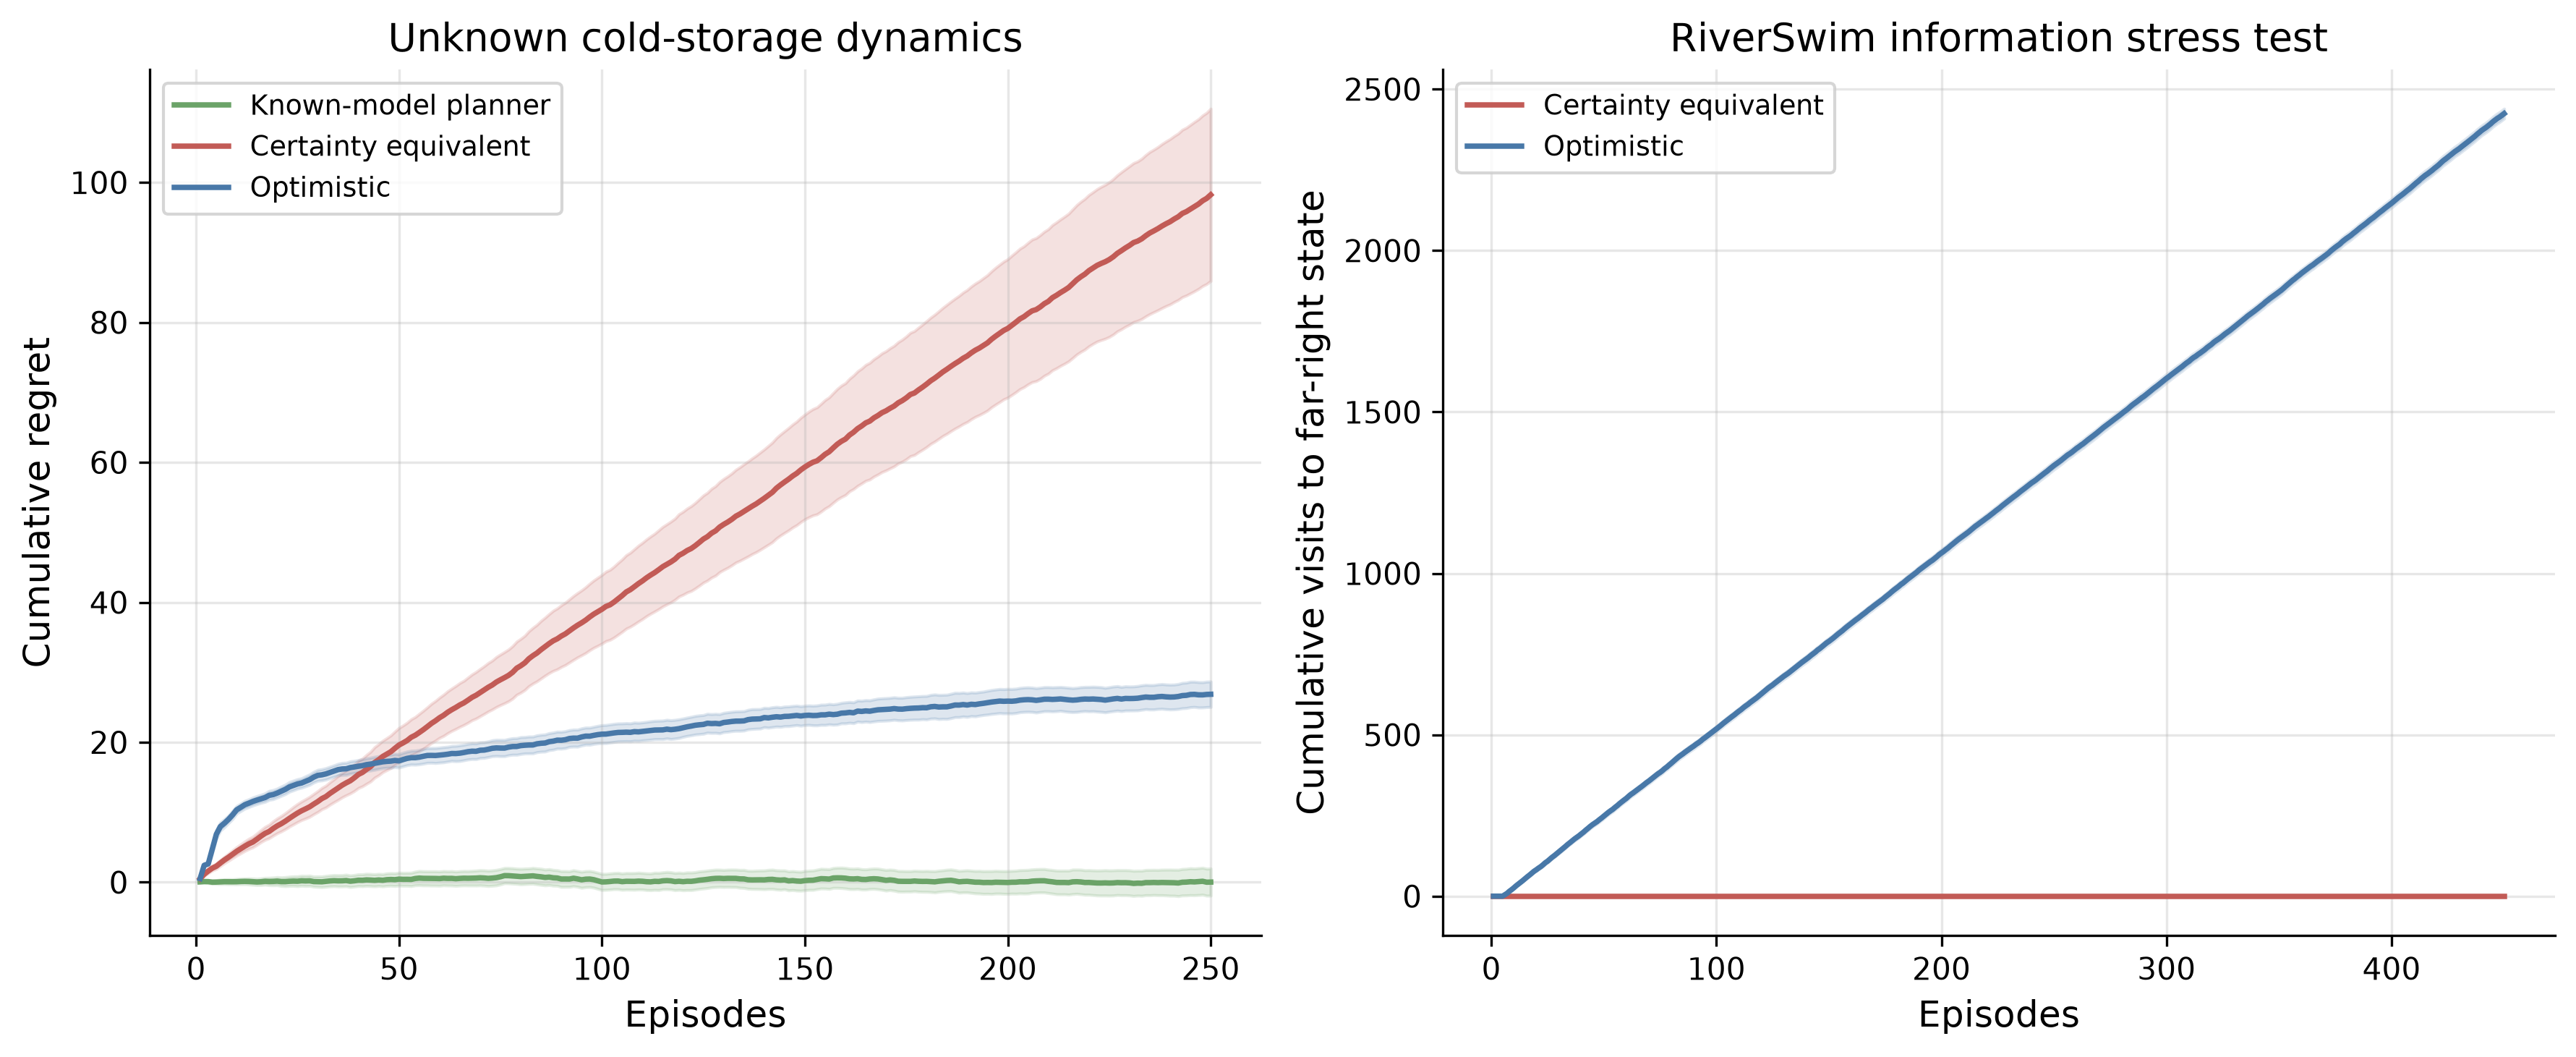
\includegraphics[width=0.96\textwidth]{../ch07a_online_optimization/sims/unknown_dynamics.png}
\caption{Known and unknown transition laws. The left panel compares three planners on identical cold-storage primitives; curves are means over 100 replications and bands are 95 percent Monte Carlo intervals. The right panel records cumulative visits to the distant rewarding state in RiverSwim.}
\label{fig:online_unknown_dynamics}
\end{figure}

The known-model and unknown-model learners solve their respective planning problems exactly. Their difference is not the accuracy of the dynamic-programming routine. It is whether the model supplied to that routine was learned from an informative sequence of actions.

\subsubsection{RiverSwim and controlled information}

The right panel isolates this mechanism in RiverSwim \citep{strehl2009interval}. The environment is a six-state chain. Moving left is easy and produces a small reward near the initial state. Moving right usually leaves the state unchanged, sometimes moves left, and only occasionally moves right. A large reward is available at the far-right state. Reaching it requires selecting the apparently unproductive right action repeatedly.

The certainty-equivalent rule uses deterministic tie-breaking and treats unvisited transitions as self-loops. It remains at the left reward and never visits the far-right state in the simulation. The optimistic rule assigns bonuses to unvisited actions and reaches the far-right state 2,424 times on average over 450 episodes. Both rules repeatedly optimize their estimated MDPs. Only one generates the data needed to revise the model.

This example distinguishes exploration from ordinary bandit feedback. In a one-period bandit, selecting an action reveals information about that action but does not change where the next decision begins. In RiverSwim, early right actions move the learner into states from which later transitions and rewards can be observed. Information is distributed along controlled paths.

\subsubsection{Regret guarantees with unknown transitions}

\citet{rosenbergMansour2019} provide the first occupancy-based extension in this sequence. They study adversarial episodic MDPs with unknown transitions and full-information losses. Their method combines online mirror descent with confidence sets for the transition law. It also permits convex performance criteria defined on an episode occupancy, extending the linear objective in equation~\eqref{eq:online_occupancy_identity}.

\citet{jinEtAl2020adversarial} consider the harder combination of unknown transitions and bandit loss feedback. A direct importance estimate based on the probability of visiting $(s,a)$ can have unbounded variance when that probability is small. Their algorithm constructs an upper bound on each occupancy probability and uses it in an optimistic loss estimator, while confidence sets control transition uncertainty.

For $K$ episodes, horizon $H$, $S$ states, and $A$ actions, their high-probability regret has order
\begin{equation}
\widetilde O\!\left(
HS\sqrt{AK}
\right),
\label{eq:online_jin_unknown_bound}
\end{equation}
where logarithmic factors are suppressed. The theorem applies to the paper's finite-horizon layered model, adversarial losses, bandit feedback, and confidence construction. It is not a guarantee for the simple bonus in equation~\eqref{eq:online_storage_bonus}.

The progression from Section~\ref{sec:online_known_transitions} can now be stated without changing vocabulary. With known $P$, the learner optimizes over the known flow set $\mathcal D(P)$. With unknown $P$, it estimates a family of plausible flow sets and must visit uncertain state-action pairs often enough for that family to contract. Online optimization remains inside the algorithm, but its feasible set and feedback are supplied by an adaptive statistical experiment.

\subsection{Current extensions as of August 2026}
\label{sec:online_current_extensions}

The classical $O(\sqrt T)$ full-information regret guarantee is now a baseline rather than a complete description of online decision problems. Current work asks whether performance can adapt to an easy realized sequence, whether the benchmark may change, how little feedback is sufficient, how constraints are enforced during learning, and how expensive each update is. The corresponding RL work asks the same questions when actions also determine state occupancies and transition data. Existing results cover selected combinations rather than the complete list.

\subsubsection{Adapting to the realized sequence}

Static regret compares with one fixed decision. When objectives change gradually, a moving benchmark $u_1,\ldots,u_T$ may be more informative:
\begin{equation}
R_T^{\mathrm{dyn}}(u_{1:T})
=
\sum_{t=1}^T f_t(x_t)
-
\sum_{t=1}^T f_t(u_t).
\label{eq:online_dynamic_regret}
\end{equation}
Without a restriction, the comparator can choose the best action separately after every round and sublinear dynamic regret is impossible. Guarantees therefore depend on a measure of change, such as path length
\begin{equation}
P_T
=
\sum_{t=2}^T\lVert u_t-u_{t-1}\rVert,
\label{eq:online_path_length}
\end{equation}
the number of switches, or the total variation of the loss functions.

\citet{liu2025nonstationary} study nonstationary bandit convex optimization under all three measures. For strongly convex losses their polynomial-time method is minimax optimal in important regimes when switch or variation budgets are known, and a bandit-over-bandit construction adapts when those budgets are unknown. Their general-convex-loss method attains stronger rates but is not polynomial-time computable. These computational qualifications matter when carrying the result into RL, where each update may already require a planning problem.

Another approach replaces variation in the minimizer by variation in gradients. For comparator $u$, define
\begin{equation}
V_T(u)
=
\sum_{t=2}^T
\left\lVert
\nabla f_t(u)-\nabla f_{t-1}(u)
\right\rVert_2^2.
\label{eq:online_gradient_variation}
\end{equation}
\citet{zhao2026gradient} obtain, for smooth convex losses, a parameter-free bound of order
\begin{equation}
\widetilde O\!\left(
\lVert u\rVert\sqrt{V_T(u)}
+
L\lVert u\rVert^2
+
G^4
\right)
\label{eq:online_gradient_variation_bound}
\end{equation}
without advance knowledge of the comparator norm, Lipschitz constant, or smoothness. The guarantee can be smaller than a horizon-only bound when gradients change little along the realized sequence.

For RL, nonstationarity can enter both rewards and transitions. A changing reward with fixed known transitions preserves one occupancy set and changes only the objective. Changing transitions move the feasible set itself and invalidate data collected under earlier laws. The second problem combines dynamic regret with model tracking and cannot be obtained by substituting a moving loss into equation~\eqref{eq:online_oreps_update}.

\subsubsection{Limited and irregular feedback}

Full-information OCO assumes that the loss function or a usable gradient is available after the decision. Applications may instead provide delayed outcomes, comparisons, censored observations, or heavy-tailed measurements.

\citet{digregorio2026probes} study a learner that normally receives full OCO feedback but has only a sublinear budget of additional noisy pairwise probes. A probe compares the losses at two points rather than returning either loss exactly. Their bound interpolates with the probe budget and deteriorates as the comparison noise approaches a fair coin.

\citet{liu2026heavytails} consider stochastic gradients with only a finite $p$th moment for $p\in(1,2]$. Under a bounded decision domain, classical methods including online gradient descent attain optimal dependence on the problem parameters without knowing $p$ and without clipping gradients. The result concerns exogenous gradient noise. In an MDP, the tail behavior can also depend on the state distribution selected by the policy, adding the occupancy issue developed above.

\subsubsection{The cost of carrying out an update}

Equation~\eqref{eq:online_projected_gradient} hides the cost of projection. Projection onto a simplex is elementary; projection onto a large routing, matching, or occupancy polytope may require a substantial optimization problem. \citet{mhammedi2025separation} replace repeated projection with a separation oracle, which either certifies feasibility or returns a separating hyperplane. Their algorithm attains
\begin{equation}
\widetilde O(\sqrt{dT}+\kappa d)
\label{eq:online_separation_bound}
\end{equation}
regret with $\widetilde O(1)$ oracle calls per round. Here $d$ is dimension and $\kappa$ measures the conditioning of the feasible set; the leading $\sqrt{dT}$ term does not depend on $\kappa$.

For the occupancy problem, an oracle call is a planning operation under the transition law. Two algorithms with the same statistical regret can therefore have very different total computation. A complete comparison reports both deployed regret and the number or cost of planning calls.

\subsubsection{Nonlinear objectives over occupancies}

Expected additive reward is linear in the occupancy:
\[
J_k(\pi)=\langle d^\pi,r_k\rangle.
\]
Some policy objectives depend nonlinearly on the distribution of visits. A public-transit operator may value total service while penalizing dispersion in waiting times across neighborhoods. A conservation planner may reward geographic coverage rather than repeated visits to the same locations. Such objectives can be written
\begin{equation}
J_k(\pi)=F_k(d^\pi),
\label{eq:online_convex_rl_objective}
\end{equation}
where $F_k$ is convex when expressed as a loss.

The online comparator becomes
\begin{equation}
\sum_{k=1}^K F_k(d^{\pi_k})
-
\min_\pi\sum_{k=1}^K F_k(d^\pi).
\label{eq:online_convex_rl_regret}
\end{equation}
With known transitions this is online convex optimization over $\mathcal D(P)$, rather than the linear special case in equation~\eqref{eq:online_mdp_occupancy_regret}. Bellman recursion generally does not apply because $F_k$ need not decompose into stage rewards.

\citet{moreno2025convexrl} study the episodic problem when transitions are unknown. Their full-information method combines mirror descent over changing estimated occupancy constraints with an exploration bonus. They also study value-only feedback, where the learner observes $F_k(d^{\pi_k})$ but not its gradient or its values at other occupancies, and adapt bandit convex-optimization methods to the MDP. The result is the direct modern extension of the chapter's known-flow reduction: nonlinearity changes the optimizer, while unknown transitions still require exploration to learn feasible flows.

\subsubsection{Resources, constraints, and safety}

Online resource allocation resembles constrained online optimization but need not be an MDP. A cloud provider that accepts jobs against a fixed capacity stock faces an online linear program: each acceptance earns value and consumes resources, but it need not change the distribution of future job types. Dual variables act as resource prices.

\citet{gao2026beyond} show that first-order dual-price methods can improve on $O(\sqrt T)$ regret when the dual problem satisfies an error-bound condition. They obtain $o(\sqrt T)$ for continuous-support arrivals and $O(\log T)$ for finite-support arrivals, beyond the nondegeneracy condition used by earlier logarithmic-regret results. These rates use structural properties of the allocation problem. They do not cover a setting in which accepting a job changes future demand or the information available about it.

General constrained OCO permits the constraint to change with the round. \citet{supantha2026constraints} bound dynamic regret and cumulative violation when both costs and constraints are adversarial and the constraint sets need not share a common feasible point. Their first method uses projection; their second is projection-free and improves violation bounds in rapidly changing environments.

In a constrained MDP, expected resource use also depends on policy-induced occupancy. Learning creates an additional safety problem because exploration itself may violate the constraint. \citet{schiffer2026safe} study a one-dimensional linear system with unknown dynamics and require the state to remain in a safe region with high probability. Their algorithm attains $\widetilde O(\sqrt T)$ regret against a class of truncated linear controllers. The one-dimensional dynamics, high-probability state constraint, and comparator class are part of the theorem.

\citet{stradi2025adversarial} consider episodic constrained MDPs with nonstationary rewards and constraints under bandit feedback. Fully adversarial rewards and constraints admit an impossibility result under the usual best-in-hindsight feasible-policy benchmark. They therefore measure the environment's departure from a stochastic problem by $C$ and obtain regret and positive constraint violation of order
\begin{equation}
\widetilde O(\sqrt T+C).
\label{eq:online_cmdp_adversarialness}
\end{equation}
The bound becomes uninformative when $C$ is of order $T$, consistently with the impossibility result.

\subsubsection{Online control with known dynamics}

Online control lies between the known-transition MDP and unknown-transition RL. A common model is
\begin{equation}
S_{t+1}=AS_t+BA_t+W_t,
\label{eq:online_linear_control}
\end{equation}
where $A$ and $B$ are known and disturbances $W_t$ may be adversarial. Actions change future states, so comparator policies must be evaluated on counterfactual trajectories. The dynamics are known, so exploration to estimate $A$ and $B$ is unnecessary.

The July 2026 preprint of \citet{xu2026counterfactual} simulates comparator policies on the revealed disturbance history and tracks their counterfactual state-action paths with a stabilizing controller. For a finite class of $N$ causal policies, the regret dependence is $\sqrt{T\log N}$ under the paper's bounded-diameter and stability conditions. The comparator policies may be nonlinear or dynamic. The result is a preprint rather than a peer-reviewed conference publication, and it assumes a known linear plant.

These extensions leave a substantial combined problem unresolved. Current theory does not provide one computationally efficient method for high-dimensional function approximation, nonlinear occupancy objectives, unknown and changing transitions, delayed or bandit feedback, and pathwise safety constraints simultaneously. Each added feature changes either the objective, the feasible occupancy set, the feedback, or the admissible exploration path.

\subsection{Technical appendix: proofs and computational details}
\label{sec:online_technical_appendix}

This section records the derivations and simulation procedures behind the chapter's main comparisons. It can be skipped on a first reading. The order follows the main text: one-period regret, chosen-action feedback, occupancy flows, the Bellman saddle problem, and unknown-transition experiments.

\subsubsection{Timing, information, and the fixed comparator}

The protocol in equation~\eqref{eq:online_static_regret} contains an information restriction that is easy to omit in an implementation. Let $\mathcal F_{t-1}$ contain all decisions, losses, and random draws observed through round $t-1$. The decision $x_t$ must be measurable with respect to $\mathcal F_{t-1}$ and any fresh randomization used at round $t$. It cannot depend on $f_t$. The loss may be selected before play begins, or it may adapt to earlier decisions, but the standard adversarial model does not allow it to inspect the learner's fresh random action before assigning the current loss.

The comparator is chosen after the sequence has been realized, but this does not give the learner advance information. It is an evaluation device. If $x^\star\in\argmin_x\sum_t f_t(x)$, regret can be written
\[
R_T=\sum_{t=1}^T\bigl[f_t(x_t)-f_t(x^\star)\bigr].
\]
The terms need not be nonnegative. The learner can outperform the best fixed decision on some rounds or even over the complete horizon because it is allowed to change decisions. A regret guarantee controls the shortfall when the fixed benchmark is better.

The horizon is also part of the protocol. The choice $\eta=D/(G\sqrt T)$ in equation~\eqref{eq:online_ogd_bound} assumes that $T$ is known. When it is not, a doubling schedule runs the method for blocks of lengths $1,2,4,\ldots$ and restarts with the step size appropriate for each block. Summing the $O(\sqrt{2^j})$ block regrets preserves an $O(\sqrt T)$ order. This distinction is operational rather than specific to RL: the same schedule can be applied to the one-period MDP update.

\subsubsection{A complete projected-gradient calculation}

For any comparator $x\in\mathcal X$, equation~\eqref{eq:online_projection_step} implies
\begin{equation}
\langle g_t,x_t-x\rangle
\leq
\frac{\lVert x_t-x\rVert_2^2-\lVert x_{t+1}-x\rVert_2^2}{2\eta}
+\frac{\eta}{2}\lVert g_t\rVert_2^2.
\label{eq:online_ogd_one_step}
\end{equation}
Summing gives
\begin{align}
\sum_{t=1}^T\langle g_t,x_t-x\rangle
&\leq
\frac{\lVert x_1-x\rVert_2^2-\lVert x_{T+1}-x\rVert_2^2}{2\eta}
+\frac{\eta}{2}\sum_{t=1}^T\lVert g_t\rVert_2^2 \nonumber\\
&\leq \frac{D^2}{2\eta}+\frac{\eta G^2T}{2}.
\label{eq:online_ogd_telescoping}
\end{align}
Convexity replaces each inner product on the left by an upper bound on $f_t(x_t)-f_t(x)$. Taking $x=x^\star$ proves equation~\eqref{eq:online_ogd_bound}. The two terms show why the step size contains $T^{-1/2}$. A smaller $\eta$ limits movement but leaves the initial-distance term large; a larger $\eta$ reacts quickly but accumulates the squared-gradient term.

In the power example, let $x_t\in[0,1]$ be the share assigned to the first contract. The two-dimensional allocation $(x_t,1-x_t)$ has scalar loss
\[
f_t(x_t)=x_t\ell_t(1)+(1-x_t)\ell_t(2),
\qquad
g_t=\ell_t(1)-\ell_t(2).
\]
The projected update is therefore
\begin{equation}
x_{t+1}=\min\{1,\max\{0,x_t-\eta[\ell_t(1)-\ell_t(2)]\}\}.
\label{eq:online_power_scalar_update}
\end{equation}
As an MDP, $x_t=\pi_t(1\mid s)$ and $1-x_t=\pi_t(2\mid s)$. Equation~\eqref{eq:online_power_scalar_update} is literally the policy update. No transition or value term is being suppressed; the episode ends after the draw.

\subsubsection{Why exponential weights has logarithmic action dependence}

The Hedge guarantee can be derived from a scalar potential. Start with weights $w_1(a)=1$ and define
\[
w_{t+1}(a)=w_t(a)e^{-\eta\ell_t(a)},
\qquad
p_t(a)=\frac{w_t(a)}{W_t},
\qquad
W_t=\sum_aw_t(a).
\]
For losses in $[0,1]$, Hoeffding's lemma gives
\begin{equation}
\log\frac{W_{t+1}}{W_t}
=
\log\sum_ap_t(a)e^{-\eta\ell_t(a)}
\leq
-\eta\langle p_t,\ell_t\rangle+\frac{\eta^2}{8}.
\label{eq:online_hedge_upper_potential}
\end{equation}
For any fixed action $a^\star$,
\begin{equation}
\log\frac{W_{T+1}}{W_1}
\geq
\log\frac{w_{T+1}(a^\star)}{A}
=
-\eta\sum_{t=1}^T\ell_t(a^\star)-\log A.
\label{eq:online_hedge_lower_potential}
\end{equation}
Combining equations~\eqref{eq:online_hedge_upper_potential} and \eqref{eq:online_hedge_lower_potential} yields
\begin{equation}
\sum_{t=1}^T\langle p_t,\ell_t\rangle
-
\sum_{t=1}^T\ell_t(a^\star)
\leq
\frac{\log A}{\eta}+\frac{\eta T}{8}.
\label{eq:online_hedge_bound}
\end{equation}
Choosing $\eta=\sqrt{8\log A/T}$ gives a bound of order $\sqrt{T\log A}$. The dependence is logarithmic because the initial potential spreads unit weight across $A$ alternatives. In the one-state MDP, the same calculation compares the sequence of stochastic policies $p_t$ with the best fixed deterministic policy.

\subsubsection{The cost of estimating an unobserved loss vector}

Unbiasedness in equation~\eqref{eq:online_importance_unbiased} is only the first property of the bandit estimator. Its conditional second moment is
\begin{align}
\mathbb E_t\!\left[\widehat\ell_t(a)^2\right]
&=
\sum_b p_t(b)
\frac{\ell_t(b)^2\indicator{b=a}}{p_t(a)^2}
=
\frac{\ell_t(a)^2}{p_t(a)}, \\
\mathbb E_t\!\left[\sum_a p_t(a)\widehat\ell_t(a)^2\right]
&=
\sum_a\ell_t(a)^2
\leq A.
\label{eq:online_bandit_second_moment}
\end{align}
The full-information analogue is at most one because $\sum_ap_t(a)\ell_t(a)^2\leq1$. This is the source of the additional factor involving $A$ in the Exp3 rate. The estimator does not create information about unselected actions; it creates an unbiased random variable whose variance accounts for their absence.

The simulated market-layout loss has a common demand component and an action-specific congestion component. It is generated before Hedge or Exp3 runs. Hedge and Exp3 therefore face the same objective sequence. Each is also evaluated as a one-period MDP policy: expected loss is $\langle p_t,\ell_t\rangle$, while realized Exp3 loss is $\ell_t(A_t)$. The plotted Exp3 regret averages the realized quantity over independent policy draws. The confidence band measures algorithmic randomization, not uncertainty about a newly sampled environment.

\subsubsection{Policy regret in the soil model}

The soil example can be calculated without simulation error. Let $F$ and $D$ denote fertile and depleted soil. The always-harvest learner begins in $F$, earns one in season one, enters $D$, and earns zero thereafter. Its $T$-season reward is
\[
G_T^{\mathrm{learner}}=1.
\]
When the rotation policy is evaluated on the learner's realized state path, it receives $1$ in the first fertile season and $0.2$ for resting in each later depleted season:
\[
G_T^{\mathrm{rotate\ on\ learner\ states}}=1+0.2(T-1).
\]
The resulting realized-state regret is $0.2(T-1)$. When rotation is deployed from the initial state, its reward sequence is $1,0.2,1,0.2,\ldots$. For even $T$,
\[
G_T^{\mathrm{rotate\ counterfactual}}=0.6T,
\qquad
R_T^{\mathrm{pol}}=0.6T-1.
\]
At $T=120$, these expressions give $23.8$ and $71.0$, respectively. Both numbers are computed from the same learner trajectory and the same policy class. Only the comparator state path changes.

This example also clarifies why policy regret is not automatically the appropriate criterion for every MDP study. If an analysis evaluates a policy from a fixed initial distribution in a stationary MDP, ordinary RL value already uses the policy's own induced path. The error occurs when online external regret is imported while holding the learner's controlled states fixed for every comparator.

\subsubsection{Occupancy correspondence}

The central known-transition statement can be separated into feasibility, policy recovery, and objective equality.

\begin{theorem}[Finite-horizon occupancy correspondence]
Fix an episodic finite MDP with initial distribution $\rho$ and transitions $P_1,\ldots,P_{H-1}$. A nonnegative array $d=(d_1,\ldots,d_H)$ is generated by a Markov policy if and only if it satisfies equations~\eqref{eq:online_flow_initial}--\eqref{eq:online_flow_transition}. For every stage-loss array $\ell$, the expected policy loss is $\langle d,\ell\rangle$.
\label{thm:online_occupancy_correspondence}
\end{theorem}

\begin{proof}
Suppose first that $d=d^\pi$. At stage one,
\[
\sum_a d_1^\pi(s,a)
=
\Pr(S_1=s)
=\rho(s).
\]
For $h\geq1$, the law of total probability gives
\begin{align*}
\sum_a d_{h+1}^\pi(s,a)
&=\Pr(S_{h+1}=s)\\
&=\sum_{s',a'}
\Pr(S_h=s',A_h=a')P_h(s\mid s',a')\\
&=\sum_{s',a'}d_h^\pi(s',a')P_h(s\mid s',a'),
\end{align*}
so every policy occupancy is feasible.

For the converse, take any feasible $d$ and define $\pi^d$ by equation~\eqref{eq:online_occupancy_policy}. Let $\mu_h(s)=\sum_a d_h(s,a)$. At stage one, feasibility gives $\mu_1=\rho$. If the process under $\pi^d$ has state distribution $\mu_h$, then
\[
\Pr(S_h=s,A_h=a)
=
\mu_h(s)\pi_h^d(a\mid s)
=d_h(s,a)
\]
at every positive-mass state. Its next-state distribution is
\[
\sum_{s',a'}d_h(s',a')P_h(s\mid s',a')
=
\sum_a d_{h+1}(s,a)
=\mu_{h+1}(s).
\]
Induction establishes that $\pi^d$ generates $d$ at every stage. Zero-mass states do not affect the induction.

Finally,
\[
\mathbb E_{\pi,P}\!\left[\sum_{h=1}^H\ell_h(S_h,A_h)\right]
=
\sum_{h,s,a}\Pr_{\pi,P}(S_h=s,A_h=a)\ell_h(s,a)
=\langle d^\pi,\ell\rangle.\qedhere
\]
\end{proof}

Summing the initial constraint over $s$ and applying the transition constraint recursively shows that
\begin{equation}
\sum_{s,a}d_h(s,a)=1
\quad\text{for every }h,
\qquad
\sum_{h,s,a}d_h(s,a)=H.
\label{eq:online_occupancy_mass}
\end{equation}
An episodic occupancy is therefore a probability distribution within each stage but has total mass $H$ across the episode. This accounts for the horizon factors in regret bounds and for the unnormalized relative-entropy expression in equation~\eqref{eq:online_flow_kl}.

Theorem~\ref{thm:online_occupancy_correspondence} proves both directions required by the reduction. Optimizing over policies cannot produce a point outside $\mathcal D(P)$, and optimizing over $\mathcal D(P)$ cannot select a flow that lacks an implementing Markov policy. The equality is stronger than a relaxation: there is no integrality or representation gap in the finite tabular model.

\subsubsection{How the O-REPS update is computed}

For known $P$, equation~\eqref{eq:online_oreps_update} is a convex program. Introduce multipliers $\alpha_1(s)$ for the initial constraints and $\alpha_{h+1}(s)$ for later flow constraints. Ignoring zero-mass boundary details, first-order conditions give an exponential tilt of the previous flow,
\begin{equation}
d_{k+1,h}(s,a)
\propto
d_{k,h}(s,a)
\exp\!\left[-\eta\widehat\ell_{k,h}(s,a)
+\alpha_h(s)
-\sum_{s'}P_h(s'\mid s,a)\alpha_{h+1}(s')\right].
\label{eq:online_oreps_tilt}
\end{equation}
The multipliers adjust the unconstrained exponential update until probability entering each state equals probability leaving the preceding layer. They play a continuation-value role inside the projection, which is why independent per-state Hedge updates do not reproduce O-REPS.

The timed-entry experiment solves the relative-entropy program directly. The computational protocol is:
\begin{algorithm}[htbp]
\caption{Known-transition occupancy update used in the timed-entry study}
\label{alg:online_known_occupancy}
\begin{algorithmic}[1]
\State Fix $P$, $\rho$, horizon $H$, and a strictly positive feasible occupancy $d_1$.
\For{day $k=1,\ldots,K$}
\State Recover $\pi_k$ from $d_k$ using equation~\eqref{eq:online_occupancy_policy}.
\State Deploy $\pi_k$ in the twelve-period MDP and record its state-action visits.
\State Reveal the day's complete loss array $\ell_k$.
\State Solve equation~\eqref{eq:online_oreps_update} subject to the fixed flow equations.
\State Evaluate the exact expected loss $\langle d_k,\ell_k\rangle$ for the regret plot.
\EndFor
\State Solve one backward-induction problem with average loss $K^{-1}\sum_k\ell_k$ to obtain the best fixed Markov policy in hindsight.
\end{algorithmic}
\end{algorithm}

The final benchmark step is valid because $P$ is common across days:
\[
\min_\pi\sum_{k=1}^KJ_k(\pi)
=
K\min_\pi\left\langle d^\pi,\frac1K\sum_{k=1}^K\ell_k\right\rangle.
\]
Backward induction and the occupancy linear program therefore compute the same comparator. The implementation evaluates both and checks their agreement rather than assuming it.

The flow residual reported in the main text is the largest absolute violation among all initial and transition equalities. The Bellman--occupancy discrepancy is the largest absolute difference between a policy's expected loss computed by backward recursion and by $\langle d^\pi,\ell_k\rangle$. Values near machine precision test the mathematical identity and the array indexing. They do not test a statistical approximation because this study uses exact transitions and full loss arrays.

\subsubsection{The mirror-descent regret step}

The optimization argument behind O-REPS is the same mirror-descent inequality used on a simplex, with $\mathcal D(P)$ replacing $\Delta(\mathcal A)$. Let $\psi$ be differentiable and strongly convex with respect to a norm $\lVert\cdot\rVert$, and let $\lVert\cdot\rVert_*$ be its dual norm. The optimality condition for equation~\eqref{eq:online_mirror_descent} implies, for every feasible $d$,
\begin{equation}
\eta\langle \widehat\ell_k,d_{k+1}-d\rangle
\leq
D_\psi(d,d_k)-D_\psi(d,d_{k+1})-D_\psi(d_{k+1},d_k).
\label{eq:online_mirror_three_point}
\end{equation}
Add and subtract $d_{k+1}$ in the loss inner product:
\begin{align}
\eta\langle\widehat\ell_k,d_k-d\rangle
&=
\eta\langle\widehat\ell_k,d_k-d_{k+1}\rangle
+\eta\langle\widehat\ell_k,d_{k+1}-d\rangle \nonumber\\
&\leq
D_\psi(d,d_k)-D_\psi(d,d_{k+1})
+\frac{\eta^2}{2}\lVert\widehat\ell_k\rVert_*^2.
\label{eq:online_mirror_one_step_bound}
\end{align}
The last step uses strong convexity to absorb $D_\psi(d_{k+1},d_k)$ and the dual-norm inequality $\langle u,v\rangle\leq\lVert u\rVert_*\lVert v\rVert$. Summing over episodes telescopes the divergences:
\begin{equation}
\sum_{k=1}^K\langle\widehat\ell_k,d_k-d\rangle
\leq
\frac{D_\psi(d,d_1)}{\eta}
+\frac{\eta}{2}\sum_{k=1}^K\lVert\widehat\ell_k\rVert_*^2.
\label{eq:online_mirror_generic_regret}
\end{equation}
The first term measures the geometric distance from the initial flow to the comparator; the second accumulates loss-estimator size. Full information uses $\widehat\ell_k=\ell_k$. Under trajectory feedback, importance weighting makes the second term larger, just as in equation~\eqref{eq:online_bandit_second_moment}.

Equation~\eqref{eq:online_mirror_generic_regret} is a template, not the stated O-REPS theorem. The constants in equations~\eqref{eq:online_oreps_full_bound}--\eqref{eq:online_oreps_bandit_bound} also use the layered MDP's mass, the particular unnormalized entropy, and a loss estimator tailored to trajectory feedback. The template identifies which parts of the proof come from online optimization: a one-step optimality condition, a telescoping divergence, and control of the estimator's dual norm. The MDP enters through the feasible flow set and the estimator's visitation probabilities.

There is also a support issue. Relative entropy is infinite when $d_h(s,a)>0$ but $d_{k,h}(s,a)=0$. O-REPS therefore begins from a feasible occupancy with suitable positive support over reachable state-action pairs, or uses an explicit exploration construction in partial-feedback settings. Positivity cannot be imposed at states that are structurally unreachable under $P$; those coordinates are removed or remain zero for every feasible occupancy.

\subsubsection{Why the myopic and per-state rules differ from occupancy learning}

The timed-entry comparison contains three restricted decision rules as well as O-REPS. Their restrictions can be stated in occupancy language.

The myopic rule chooses
\[
a_{k,h}^{\mathrm{myopic}}(s)
\in\argmin_a\ell_{k,h}(s,a).
\]
It returns a feasible policy and therefore a feasible occupancy, but it does not choose that occupancy by minimizing total episode loss. The transition response enters only after the pointwise actions have been selected.

The state-blind rule restricts policies to
\[
\pi_{k,h}(\mathrm{admit}\mid s)=p_k
\quad\text{for every }h,s.
\]
It accounts for neither state-specific immediate effects nor the transition response. Per-state Hedge enlarges the class to separate probabilities $p_k(s)$ but updates each from the local loss pair. It produces a valid Markov policy, yet its update treats observations at a state as if changing its action probability affected no later state frequencies.

O-REPS chooses directly within $\mathcal D(P)$. A change in admission probability at a quiet state must be accompanied by the downstream busy and crowded mass implied by $P_1$. This is the precise sense in which the RL and online-optimization representations are the same problem in this experiment: backward induction evaluates a policy using continuation losses, while the occupancy program assigns the corresponding downstream probability mass before taking the loss inner product.

\subsubsection{Deriving the discounted Bellman programs}

Start from the normalized discounted flow identity. For any policy occupancy $d^\pi_\rho$,
\begin{align}
\sum_a d^\pi_\rho(s,a)
&=(1-\gamma)\rho(s)
+(1-\gamma)\sum_{t=1}^\infty\gamma^t\Pr(S_t=s) \nonumber\\
&=(1-\gamma)\rho(s)
+\gamma\sum_{s',a'}P(s\mid s',a')d^\pi_\rho(s',a').
\label{eq:online_discounted_flow_derivation}
\end{align}
This gives the constraints in equation~\eqref{eq:online_discounted_primal}. Conversely, normalizing a feasible $d$ within each state produces a stationary policy whose discounted occupancy is $d$, by the same fixed-point argument as the finite-horizon proof.

Assign a multiplier $V(s)$ to each flow equality and write the primal Lagrangian:
\begin{align}
L(V,d)
&=
\sum_{s,a}d(s,a)r(s,a)
+\sum_sV(s)\left[(1-\gamma)\rho(s)
+\gamma\sum_{s',a'}P(s\mid s',a')d(s',a')
-\sum_a d(s,a)\right] \nonumber\\
&=
(1-\gamma)\sum_s\rho(s)V(s)
+\sum_{s,a}d(s,a)
\left[r(s,a)+\gamma\sum_{s'}P(s'\mid s,a)V(s')-V(s)\right].
\label{eq:online_bellman_lagrangian_derivation}
\end{align}
If $d\geq0$ is otherwise unrestricted, the supremum over $d$ is finite only when every bracketed Bellman advantage is nonpositive. These are exactly the inequalities in equation~\eqref{eq:online_discounted_dual}. Under those inequalities, the maximizing choice contributes no positive violation, leaving the dual objective $(1-\gamma)\rho^\top V$. This derives the dual rather than postulating it from the Bellman equation.

Complementary slackness adds the policy statement. If $d^\star(s,a)>0$, then
\[
V^\star(s)=r(s,a)+\gamma\sum_{s'}P(s'\mid s,a)V^\star(s').
\]
Thus actions used by the optimal occupancy maximize the Bellman right-hand side. The occupancy and value programs are not separate characterizations; their optimality conditions are the Bellman equation on the support of the optimal policy.

\subsubsection{The two-player regret calculation}

The saddle-gap bound in equation~\eqref{eq:online_saddle_regret} follows directly from the definitions of regret. The minimizing player's regret gives, for every $V$,
\begin{equation}
\sum_{n=1}^N L(V_n,d_n)
-
\sum_{n=1}^N L(V,d_n)
\leq R_N^V.
\label{eq:online_value_player_regret}
\end{equation}
The maximizing player's regret gives, for every $d$,
\begin{equation}
\sum_{n=1}^N L(V_n,d)
-
\sum_{n=1}^N L(V_n,d_n)
\leq R_N^d.
\label{eq:online_occupancy_player_regret}
\end{equation}
Adding and using bilinearity,
\[
L(\bar V_N,d)-L(V,\bar d_N)
\leq\frac{R_N^V+R_N^d}{N}.
\]
Taking the maximum over $d$ and the minimum over $V$ proves equation~\eqref{eq:online_saddle_regret}. Averaging is essential: the argument controls $L(\bar V_N,d)$ and $L(V,\bar d_N)$, not necessarily the final pair $(V_N,d_N)$.

The Engine Replacement comparison keeps this numerical role separate from online deployment. Both solvers know the exact reward and transition matrices. Value iteration uses the contraction special to discounted dynamic programming. The no-regret solver treats the two sides of equation~\eqref{eq:online_bellman_lagrangian} as repeated linear objectives. Its slower convergence in Figure~\ref{fig:online_bellman_solver} is consistent with using a general saddle method on a problem for which a stronger contraction algorithm is available.

The generic two-player certificate in the figure is also expected to be looser than the policy-value gap. It is uniform over the chosen compact value and occupancy domains, whereas policy loss depends only on the extracted policy and initial distribution. The Cheng et al. reduction constructs a comparator tailored to policy performance; equation~\eqref{eq:online_cheng_approximation} should not be read as a statement that every generic saddle diagnostic equals policy regret.

\subsubsection{Unknown transitions as an adaptive sampling problem}

For a fixed state-action pair, equation~\eqref{eq:online_empirical_transition} is an ordinary multinomial estimate conditional on the number of visits $N_k(s,a)$. The visit count is not ordinary fixed-design sample size. It satisfies
\[
N_k(s,a)=\sum_{j<k}\sum_{h=1}^H\indicator{S_{j,h}=s,A_{j,h}=a},
\]
and is therefore generated by earlier policies and transitions. Two algorithms can have the same total number of periods but radically different sample sizes for a transition row.

Confidence sets turn the dependence into a planning object. A schematic row-wise set is
\begin{equation}
\mathcal P_k(s,a)
=
\left\{p\in\Delta(\mathcal S):
\lVert p-\widehat P_k(\cdot\mid s,a)\rVert_1
\leq c\sqrt{\frac{S\log(KSA/\delta)}{\max\{1,N_k(s,a)\}}}
\right\}.
\label{eq:online_transition_confidence_set}
\end{equation}
The constant and radius depend on the concentration result used by a particular algorithm. The common structure is what matters here: an unvisited pair has a wide set, and repeated visits shrink it. Optimistic planning chooses a model or value within the set that makes uncertain actions attractive enough to be sampled.

A generic optimistic model-based loop can be written as Algorithm~\ref{alg:online_unknown_transition}. It is deliberately schematic. A theorem must specify the confidence radius, how optimism is optimized jointly over plausible transition rows, whether losses are fully observed or importance weighted, and how failure probabilities are combined across episodes.

\begin{algorithm}[htbp]
\caption{Schematic occupancy-based learning with unknown transitions}
\label{alg:online_unknown_transition}
\begin{algorithmic}[1]
\State Initialize transition counts $N_1(s,a,s')=0$ and an exploration-support rule.
\For{episode $k=1,\ldots,K$}
\State Form empirical transitions $\widehat P_k$ from the accumulated counts.
\State Construct plausible transition rows $\mathcal P_k(s,a)$ using visit-dependent radii.
\State Combine the current online loss update with optimism over plausible transitions.
\State Solve the resulting finite-horizon planning or occupancy problem and recover $\pi_k$.
\State Deploy $\pi_k$ for one episode; observe visited losses and transitions.
\State Update $N_{k+1}(s,a,s')$ only for the transitions actually observed.
\EndFor
\end{algorithmic}
\end{algorithm}

The known-transition algorithm in Algorithm~\ref{alg:online_known_occupancy} begins each update with one fixed feasible set $\mathcal D(P)$. Algorithm~\ref{alg:online_unknown_transition} instead constructs a data-dependent family
\[
\bigcup_{P'\in\mathcal P_k}\mathcal D(P').
\]
Optimism selects a favorable member of that family while the online loss term controls performance across episodes. Deployment then changes both cumulative loss and the family available at the next episode. This feedback from the decision to the next feasible-set estimate is absent from ordinary OCO with a known constraint set.

The same loop can be pessimistic rather than optimistic in offline RL, where no new transitions can be collected. Pessimism avoids policies whose value relies on unsupported pairs. Online RL has the additional option of visiting such pairs and reducing their uncertainty. The direction of the adjustment reflects whether the data-collection policy can still be changed.

The cold-storage bonus in equation~\eqref{eq:online_storage_bonus} is deliberately simpler than a theorem-level confidence algorithm. It tests the mechanism on a transparent three-state model. All three methods solve a finite-horizon planning problem before each episode. Their information differs:
\begin{enumerate}
\item The known-model planner receives the true $P_{\mathrm{monitor}}$ and $P_{\mathrm{service}}$.
\item Certainty equivalence plans under the empirical rows $\widehat P_k$ with self-loops at unvisited pairs.
\item The optimistic learner uses the same empirical rows and subtracts a visit-count bonus from loss.
\end{enumerate}
The known-model method is both an RL planner and the optimizer over the true occupancy set. The two unknown-model methods are RL algorithms because their policies control the transition samples used in later plans. Figure~\ref{fig:online_unknown_dynamics} compares these formulations on the same true MDP rather than comparing unrelated applications.

RiverSwim removes maintenance-specific details while preserving the information mechanism. The far-right reward can be estimated only after a sequence of right actions carries the process across the chain. A learner that repeatedly solves a self-loop model can be exactly optimal for that estimated model and still collect no evidence that refutes it. The example therefore separates three errors:
\begin{align*}
\text{planning error} &:\ \text{failure to solve the supplied model},\\
\text{estimation error} &:\ \widehat P_k\text{ differs from }P,\\
\text{exploration error} &:\ \text{the policy supplies too little data for the difference to shrink}.
\end{align*}
The certainty-equivalent rule has zero planning error in the simulation. Its large learning error comes from the other two terms.

\subsubsection{Simulation design and numerical checks}

Each experiment is paired: an online-optimization description and an RL description use identical primitive data. Table~\ref{tab:online_paired_studies} states the equality or contrast being checked.

\begin{table}[htbp]
\centering
\caption{Paired formulations used in the simulation suite.}
\label{tab:online_paired_studies}
\footnotesize
\begin{tabular}{@{}p{0.16\textwidth}p{0.47\textwidth}p{0.25\textwidth}@{}}
\toprule
Study & Two descriptions of the same primitives & Check \\
\midrule
Power procurement & Simplex allocation; one-state, one-period MDP policy & Decisions and expected losses coincide \\
Market layout & Full-vector or selected-coordinate optimization; one-period MDP with full or bandit feedback & Same objective, different estimator variance \\
Soil management & External or policy comparator; two-state controlled process & Comparator state path changes regret \\
Timed entry & Linear optimization over $\mathcal D(P)$; twelve-period known-transition MDP & Flow and Bellman values coincide \\
Engine replacement & Two-player online saddle updates; fixed discounted MDP & Extracted-policy gap is controlled by optimization \\
Cold storage & Optimization over an estimated flow model; unknown-transition episodic RL & Exact planning does not replace exploration \\
\bottomrule
\end{tabular}
\end{table}

Table~\ref{tab:online_simulation_calibration} records the sample sizes used for the frozen figures. The horizons were selected before examining the plotted results. Longer horizons are used when the target is an asymptotic diagnostic; multiple independent replications are used only when feedback or transitions make the reported outcome random.

\begin{table}[htbp]
\centering
\caption{Simulation horizons, replications, and sources of randomness.}
\label{tab:online_simulation_calibration}
\small
\begin{tabular}{p{0.23\textwidth}p{0.18\textwidth}p{0.16\textwidth}p{0.32\textwidth}}
\toprule
Study & Horizon & Replications & Random component \\
\midrule
Power procurement & $T=50$ to $2{,}000$ & One per horizon & None; alternating losses are deterministic \\
Market layout & $T=1{,}500$ & 200 & Exp3 action draws; common pre-generated loss sequence \\
Soil management & $T=120$ & One & None; states and policies are deterministic \\
Timed entry & $K=300$, $H=12$ & One & Exact expected losses; simulated visits only for summaries \\
Engine replacement & $N=5{,}000$ & One & None; exact model gradients \\
Cold storage & $K=250$, $H=12$ & 100 & Policy actions and true state transitions \\
RiverSwim & $K=450$, $H=20$ & 100 & Policy actions and chain transitions \\
\bottomrule
\end{tabular}
\end{table}

\paragraph{Power and market benchmarks.}
For one-period problems, the hindsight benchmark is obtained by summing the complete loss matrix down the time dimension and selecting its smallest column. This remains valid for Exp3 even though Exp3 does not observe that matrix: the benchmark belongs to evaluation and can use the pre-generated sequence. For the alternating power sequence, both fixed contracts lose $T/2$ when $T$ is even. The benchmark is therefore known analytically and checks the numerical column-sum calculation.

\paragraph{Soil benchmark.}
There are four deterministic stationary Markov policies because two actions are available in each of two states. The program enumerates all four. For realized-state external regret, every policy is evaluated on the always-harvest state sequence. For policy regret, each policy is simulated from fertile soil under its own actions. Enumeration makes the change of comparator explicit and avoids an optimization approximation.

\paragraph{Timed-entry benchmark.}
The best fixed Markov policy minimizes the sum of all 300 expected episode losses. Because transitions do not change by day and expected loss is linear in $\ell_k$, the comparator is obtained by solving one finite-horizon MDP under the average loss array. The implementation separately forms its occupancy and checks the objective against backward induction. The policy is allowed to depend on period and crowding state, but not on the day index $k$.

\paragraph{Engine benchmark.}
The exact discounted values in Section~\ref{sec:online_engine_saddle} are rational numbers for the stated calibration. The optimal policy can also be verified by comparing the two Bellman action values at each state. Both numerical solvers are evaluated against this fixed solution. The saddle method is not allowed a different reward normalization or initial distribution.

\paragraph{Cold-storage and RiverSwim benchmarks.}
The known-model cold-storage policy is computed by backward induction under the true transition matrices before each replication. Its expected loss supplies the comparator; trajectory randomness can therefore make a realized cumulative regret slightly negative. RiverSwim reports visits rather than regret because the intended diagnostic is whether the distant information-bearing state is reached. The environment and episode budget are identical for certainty equivalence and optimism.

The exogenous loss or reward sequence is generated once before methods are run whenever the environment changes across rounds. Stochastic methods receive independent random-number streams. This prevents a method that happens to draw favorable early outcomes from changing the objective sequence faced by another method. In the known-transition occupancy study, expected policy losses are evaluated exactly; trajectory draws are used only for occupancy summaries. In the unknown-transition study, trajectories are essential because they generate the estimated model.

For Monte Carlo outcome $Y_1,\ldots,Y_M$, figures report the sample mean and the pointwise interval
\begin{equation}
\bar Y\ \pm\ 1.96\frac{s_Y}{\sqrt M},
\label{eq:online_monte_carlo_interval}
\end{equation}
where $s_Y$ is the sample standard deviation across independent algorithm replications. These are Monte Carlo intervals for the plotted mean, not confidence intervals for a structural parameter. Temporal points within a replication are dependent, so they are not treated as independent observations.

The suite performs four deterministic checks before producing figures:
\begin{enumerate}
\item The one-period allocation and MDP-policy implementations agree at every update.
\item Every computed episodic occupancy satisfies initial and transition flow constraints.
\item Bellman recursion and the occupancy inner product agree for the same timed-entry policy.
\item The Engine Replacement optimal policy and values agree with the shared implementation used earlier in the book.
\end{enumerate}
The first three residuals are at floating-point precision in the reported run. The fourth prevents the reused MDP from drifting to a new calibration inside this chapter.

Regret plots include more than one normalization. $R_T/T$ answers whether average excess loss is vanishing. $R_T/\sqrt T$ is useful for detecting gross incompatibility with a square-root scale over the simulated horizons. Neither plot establishes a rate: finite-sample curvature, tuning, and lower-order terms can all mimic a slope. The theoretical rates retain the assumptions stated with their source results.

\subsubsection{Reproduction files}

All six figures and the numerical table are produced by
\begin{center}
\texttt{ch07a\_online\_optimization/sims/online\_optimization\_rl.py}.
\end{center}
The script imports the Engine Replacement primitives from \texttt{sims/engine.py}; it does not redefine them. The saved standard output records seeds, horizons, replication counts, final regrets, standard errors, flow residuals, and Bellman--occupancy discrepancies. The chapter figures are generated files rather than manually edited graphics.

The public simulation check runs the lightweight test suite against the same functions used to make the figures. In particular, it asserts exact one-period equality, the analytically implied gap between realized-state and policy regret, finite-horizon flow conservation, Bellman--occupancy agreement, and convergence of the Engine Replacement diagnostics. These checks concern implementation consistency. They do not convert the illustrative optimistic bonuses into implementations of the source papers' algorithms.

\subsection{What carries from online optimization to RL}
\label{sec:online_synthesis}

The connection can be summarized as a sequence of model changes.

With one state and one period, a stochastic policy is an action distribution. Online linear optimization and the MDP have the same decision, expected reward, update, and fixed-policy regret.

With chosen-action feedback, the mathematical objective remains the same but missing loss coordinates must be estimated. This is the adversarial bandit problem. It is still a one-period MDP, so no action changes a later state.

With several periods and known transitions, a policy induces a state-action occupancy satisfying linear flow equations. Expected episode loss is linear in that occupancy, and regret against the best fixed Markov policy is online linear optimization over $\mathcal D(P)$. The state path has not disappeared; it has been incorporated into the feasible decision.

For one fixed discounted MDP, the Bellman primal and dual define a saddle problem. No-regret algorithms can solve that saddle problem, and their average regret bounds the performance of an extracted policy under the assumptions of the reduction. Here online learning is a numerical method rather than the environment's evaluation protocol.

With unknown transitions, the occupancy set is not available in advance. Policies determine which transitions are sampled, so an RL algorithm must combine optimization with estimation and exploration. Exact optimization under an uninformative estimated model can coexist with large policy error.

These statements do not cover every use of online learning in RL. Policy-gradient and natural-gradient methods use related optimization geometry inside a fixed policy class and are treated in Section~\ref{sec:policy_gradient}. Offline RL in Section~\ref{section:offline_rl} removes control over data collection. Adaptive experimentation in Section~\ref{section:adaptive_experiments} distinguishes welfare during an experiment from inference after adaptive assignment. The narrower conclusion of this chapter is that online optimization supplies exact representations and reusable algorithms at particular points in the RL problem, while controlled states and controlled information determine where those representations stop being complete.
